\documentclass{llncs}

\makeatletter
\newif\if@restonecol
\makeatother
\let\algorithm\relax
\let\endalgorithm\relax


\usepackage[linesnumbered,ruled,vlined]{algorithm2e}
\usepackage{epsfig}
\usepackage{graphicx}
\usepackage{amsfonts}
\usepackage{enumerate}
\usepackage{dsfont}
\usepackage{amsmath}
\usepackage{url}
\usepackage{amssymb}
\usepackage{ifthen}
\usepackage{array}
\usepackage[table]{xcolor}


%%%%%%%%%%%%%%%%%%%%%%%%%%%%%%%%%%%%%%%%%%%%%%
% math macro
%%%%%%%%%%%%%%%%%%%%%%%%%%%%%%%%%%%%%%%%%%%%%%
\newcommand{\inp}{x}
\newcommand{\inpseq}{{\bf x}}
\newcommand{\f}{{\bf f}}
\newcommand{\q}{{\bf q}}
\newcommand{\blab}{{\bf \lab}}
\newcommand{\lab}{y}
\newcommand{\labs}{{\bf y}}
\newcommand{\nlab}{{\bar y}}
\newcommand{\loss}{L}
\newcommand{\expect}[1]{\mathbb{E}_{X,Y}\bigl[#1 \bigr]}

\newcommand{\fscore}{f}
\newcommand{\score}{s}
\newcommand{\SGDloss}{L_\obs(\fscore_{w(t)}(\obs_t), \labs_t)}
\newcommand{\len}[1]{{[#1]}}
\newcommand{\pair}[1]{(\inpseq_{#1},\lab_{#1})}
\newcommand{\npair}[1]{(\bar \inpseq_{#1},\bar \lab_{#1})}
\newcommand{\pairloss}{l_p(\fscore_w(\inp_i)-\fscore_w(\bar \inp_j))}
\newcommand{\pairlossArg}[1]{l_p({#1})}
\newcommand{\slossnew}{\Psi}
\newcommand{\bbeta}{\boldsymbol{\beta}}
\newcommand{\bs}{{\bf s}}
\newcommand{\boldr}{{\bf r}}

\newcommand{\qm}{{\tt r}}

\newcommand{\pospart}[1]{\left [ #1 \right ]_+}

%%%%%%%%%%%%%%%%%%%%%%%%%%%%%%%%%%%%%%%%%%%%%%%%%%%%%%
%   framework
%%%%%%%%%%%%%%%%%%%%%%%%%%%%%%%%%%%%%%%%%%%%%%%%%%%%%%

\newcommand{\lenq}[1]{|#1|}

\newcommand{\subsetOfQuery}[1]{{\cal S}(#1)}
\newcommand{\set}[1]{\left \{ #1 \right \}}
 \newcommand{\sset}[1]{\bigl \{ #1 \bigr \}}
\newcommand{\bigpospart}[1]{\Big [ #1 \Big ]_+}
\newcommand{\norm}[1]{\left | \left | #1 \right | \right |}
\newcommand{\indic}[1]{I_{\set{#1}}}
\newcommand{\expobs}{\expectation_{(\obs, \rels) \sim \mu}}

\newcommand{\expmu}{\expectation_{\inpseqb \sim \mu}}
\newcommand{\empexpmu}{\empexpectation_{\inpseqb \sim \trset}}
\newcommand{\expnu}{\expectation_{\inp \sim \nu}}

\DeclareMathOperator*{\argmax}{arg\,max}
\DeclareMathOperator*{\argmin}{arg\,min}
\DeclareMathOperator*{\argsort}{arg\,sort}
\DeclareMathOperator{\indicc}{I\!I}
\DeclareMathOperator{\nindicc}{I\!I\!I}
\DeclareMathOperator{\dist}{d}
\DeclareMathOperator*{\expectation}{\mathbb{E}}

\newcommand{\probasobs}{\probas\left({\cal S}\right)}
\newcommand{\expxy}{\expectation_{X,Y}}
\newcommand{\expx}{\expectation_{X}}

%%%%%%%%%%%%%%%%%%%%%%%%%%%%%%%%%%%%%%%%%%%%%%%%%%%%%%%%%%%%%%%%%%%%%
% textimage retrieval macro
%%%%%%%%%%%%%%%%%%%%%%%%%%%%%%%%%%%%%%%%%%%%%%%%%%%%%%%%%%%%%%%%%%%%%
\newcommand{\params}{{\bf w}}
\newcommand{\trset}{S}
\newcommand{\alts}{{\bf X}}
\newcommand{\alt}{X}
\newcommand{\emploss}{\hat{R}^{\rerr}(\score, S)}
\newcommand{\dotp}[2]{\left<#1, #2\right>} %dot product
\newcommand{\intint}[2]{\set{#1, ..., #2}}%{\left \{#1..#2\right \}}
\newcommand{\sign}{\mbox{sign}}
%\newcommand{\pospart}[1]{\left [ #1 \right ]_+}
\renewcommand{\Re}{\mathbb{R}}
%\DeclareMathOperator{\indic}{I}
\DeclareMathOperator*{\empexpectation}{\hat{\mathbb{E}}}
\newcommand{\empexpobs}{\empexpectation_{(\obs, \rels) \sim \trset}}
\newcommand{\rel}{y}
\newcommand{\nrel}{{\bar y}}

% Spaces
\newcommand{\fspace}{{\cal F}}
\newcommand{\hfspace}{{\cal H}}
\newcommand{\inpspace}{{\cal X}}
\newcommand{\supspace}{{\cal Y}}
\newcommand{\distspace}{{Pr(X,Y)}}
\newcommand{\alldistspace}{{\cal D}}


%%%%%%%%%%%%%%%%%%%%%%%%%%%%%%%%%%%%%%%%%%%%%%
% code for formatting comments
%%%%%%%%%%%%%%%%%%%%    BEGIN  %%%%%%%%%%%%%%%%%%%%
\newboolean{showcomments}
\setboolean{showcomments}{false}

\ifthenelse{\boolean{showcomments}}
{ \newcommand{\mynote}[2]{
    \fbox{\bfseries\sffamily\scriptsize#1}
    {\small$\blacktriangleright$\textsf{\emph{#2}}$\blacktriangleleft$}}}
{ \newcommand{\mynote}[2]{}}

\newcommand{\karine}[1]{\mynote{Karine}{#1}}
\newcommand{\pierre}[1]{\mynote{Pierre}{#1}}
\newcommand{\seb}[1]{\mynote{S\'ebastien}{#1}}
\newcommand{\guthemberg}[1]{\mynote{Guthemberg}{#1}}
\newcommand{\david}[1]{\mynote{David}{#1}}
%%%%%%%%%%%%%%%%%%%%    END  %%%%%%%%%%%%%%%%%%%%


%%%%%%%%%%%%%%%%%%%%%%%%%%%%%%%%%%%%%%%%%%%%%%
% code for formatting paper to gain space
%%%%%%%%%%%%%%%%%%%%    BEGIN  %%%%%%%%%%%%%%%%%%%%
%\usepackage{setspace}
%\renewcommand{\baselinestretch}{0.95}
%\addtolength{\topmargin}{-.2cm} \addtolength{\textheight}{.4cm}
%\addtolength{\oddsidemargin}{-.1cm}\addtolength{\textwidth}{.2cm}
%\sloppy
%\parindent=0pt
%
%\hbadness=6400
%\vbadness=3200
%
%
%%%%%%%%
%
%\floatsep 10mm plus 4pt minus 4pt % Space between adjacent floats moved
%\floatsep 3mm plus 4pt minus 4pt % Space between adjacent floats moved
%                                  % to top or bottom of text page.
%\textfloatsep=\floatsep           % Space between main text and floats
%                                  % at top or bottom of page.
%\intextsep=\floatsep              % Space between in-text figures and
%                                  % text.
%%%%%%%%%%%%%%%%%%%%%   END  %%%%%%%%%%%%%%%%%%%%%


\begin{document}

\title{Boosting Streaming Video Delivery with WiseReplica}

%\author{\IEEEauthorblockN{Guthemberg Silvestre\IEEEauthorrefmark{1}\IEEEauthorrefmark{2}, Karine Pires\IEEEauthorrefmark{1}, David Buffoni\IEEEauthorrefmark{1}, S\'{e}bastien Monnet\IEEEauthorrefmark{1} and Pierre Sens\IEEEauthorrefmark{1}}
%\IEEEauthorblockA{\IEEEauthorrefmark{1}LIP6/UPMC/CNRS/INRIA \\
%4 place Jussieu - 75005 Paris - France. \\
%Email: \{firstname.lastname\}@lip6.fr}
%\IEEEauthorblockA{\IEEEauthorrefmark{2}Orange Labs \\
%38-40 rue du G\'en\'eral Leclerc, 92130 Issy -- France.}
%}

\author{Guthemberg Silvestre\inst{1} \and David Buffoni\inst{2} \and  Karine Pires\inst{2} \and S\'{e}bastien Monnet\inst{2} \and Pierre Sens\inst{2}}

\institute{CNRS, LAAS, 7 avenue du colonel Roche, F-31400 Toulouse, France \
\email{gdasilva@laas.fr} \
 \and UPMC Sorbonne Universit\'es, LIP6, CNRS, INRIA, 4 Place Jussieu, Paris, France \
\email{\{david.buffoni,karine.pires,sebastien.monnet,pierre.sens\}@lip6.fr} }

\maketitle

\begin{abstract}

%specific ICNP note: abstract is limited to 200 words.
Streaming video consumption has risen sharply over the last years. Not only has that reshaped the Internet traffic, it has also changed the manner of watching videos. Users are progressively moving from the old-fashioned scheduled television to video-on-demand (VoD) services. As broadcasting future seems to be online, customers have become more sensitive to VoD quality, expecting ever-higher bitrates and lower rebuffering. In this context, average bitrate is a key quality of service (QoS) metric. Therefore, content delivery networks (CDNs) and content providers must be committed to enforcing average bitrate through service-level agreement (SLA) contracts. Adaptive content replication is a promising technique towards this goal. However, this still offers a major challenge for CDN providers, particularly as they aim to avoid waste of resources. In this work, we introduce WiseReplica, an adaptive replication scheme for peer-assisted VoD systems that enforces the average bitrate for Internet videos. Using an accurate machine-learned ranking, WiseReplica saves storage and bandwidth from the vast majority of non-popular contents for the most watched videos. Simulations using YouTube traces suggest our approach meets users expectations efficiently.  Compared to caching, WiseReplica reduces the required replication degree for the most-watched videos by two orders of magnitude, and under heavy load, it increases the average bitrate by roughly 85\%.

\end{abstract}

\begin{keywords} 
Peer-to-peer (P2P), video on-demand (VoD), caching, replication, service-level agreement (SLA), prediction.
\end{keywords}

%\begin{IEEEkeywords}
%Peer-to-peer, video on-demand (VoD), caching, replication, SLA, prediction.
%\end{IEEEkeywords}
%\IEEEpeerreviewmaketitle

\section{Introduction}

The increasing consumption of Internet videos has made fundamental changes in the Internet traffic and consumers' behaviour. Cisco System, Inc\footnote{Cisco Visual Networking Index: Forecast and Methodology, 2013-2018. www.cisco.com, 2014.} forecasts that the sum of all forms of video traffic will be in the range of 80 to 90 percent of global consumer traffic by 2018, including video on-demand (VoD), live streaming, and peer-to-peer (P2P) file sharing. In fact, as the Internet access has become ubiquitous, continuously faster, and cheaper, streaming video has become mainstream. Users are progressively moving from the old-fashioned scheduled television to VoD services. This contributes to increase the expectations of consumers on Internet video delivery. 

Since broadcasting future seems to be online, customers have become more sensitive to VoD quality, expecting ever-higher bitrates and lower rebuffering. Contrary to many traditional workloads, e.g. social network messaging or search engines, specifying just latency as quality of service (QoS) metric does not suffice. Instead, streaming traffic requires proper average bitrate to avoid rebuffering and improve user experience. For example, Dobrain \emph{et al.}\cite{Dobrian_sigcomm_2011} found that a 1\% increase in buffering ratio can reduce the consumer's expected viewing time by more than three minutes. This suggests that service-level agreement (SLA) contracts must include bitrate as a key QoS metric. 

Yet, current Content Delivery Networks (CDN) platforms are not ready to fulfil the requirements of the increasing demand for VoD services and meet consumers' expectations. Through fine-grained client-side measurements from over 200 million client viewing sessions, Liu \emph{et al.}\cite{Liu_sigcomm_2012} showed that 20\% of these sessions experience a rebuffering ratio of at least 10\%, 14\% of users have to wait more than 10 seconds for video to start up, more than 28\% of sessions have an average bitrate less than 500Kbps, and 10\% of users fail to see any video at all.

To deal with these issues, CDN providers have started to combine
datacenters and edge network resources in hybrid
designs\footnote{Akamai acquires Red
  Swoosh. http://www.akamai.com/html/about/ press/releases/
  2007/press\_041207.html, April 2007.}. This includes
\emph{peer-assisted VoD systems}~\cite{profitable_vod_sigcomm_07}
whose deployment requires hybrid CDN platforms. The aim of
peer-assisted VoD systems is to take advantage of both
infrastructure-based resources and P2P communication facilities. Huang
\emph{et al.}~\cite{profitable_vod_sigcomm_07} suggest the use of
peer-assisted VoD systems to improve resource allocation for Internet video delivery. They argue that devices on edge networks, e.g. set-top-boxes, contribute with storage and bandwidth to video delivery, reducing dramatically the burden on infrastructure-based servers, and cutting operations costs. Many recent studies~\cite{parvez_bittorrent_analysis_sigmetrics08,huang2008challenges_sigcomm08,pavod_icnp12} confirm that exploring peer-assisted VoD system permits enhancing resource allocation for streaming videos, but none has properly evaluated the performance of video delivery regarding SLA enforcement. 

In fact, there exists an increasing need for more research in easy-to-deploy, self-adapting techniques for ensuring tough QoS guarantees brought by the cloud paradigm. However, efficient resource allocation on hybrid CDNs to meet user expectations imposes big challenges, particularly for resource-hungry services as VoD. 
This paper identifies \emph{adaptive content replication} as one of such challenges. Adaptive replication plays an important role on the content availability of distributed systems, contributing directly to both storage and bandwidth provision. As the popularity of a video varies, the number of replicas, or peers serving that video, must be adapted accordingly. Generally speaking, the faster and more precise the replication scheme reacts to changes on videos demand, the better is the resource allocation and content availability. 

Considering average bitrate as target QoS metric, we make a case for a
SLA-driven replication scheme named WiseReplica that allows us to meet
users' expectations in peer-assisted VoD system properly. We assume
the system must enforce the right average bitrate for each video
through SLA contracts. Our ultimate goal is two-fold: (i) to prevent
SLA violations and (ii) to reduce the number of video replicas. To
perform efficient Internet video replication, WiseReplica relies on a
novel, accurate machine-learned ranking of Internet videos. To rank
video in order of demand,  our prediction model encompasses multiple
measurements of Internet video activity in peer-assisted VoD system,
including active viewers, video duration, average serving time, and
mean time between requests view. The use of this prediction model in
WiseReplica provides the ability to adapt the replication degree of videos dynamically according to their encoding settings and popularity, reducing storage usage and enhancing network provision.  We make two main contributions:

\noindent
\textbf{Investigate how predictable is a ranking of Internet videos.} \ We design a learning model to capture the dynamic behaviour of streaming video demand. The model makes predictions based on lightweight measurements of the request arrival process. Using a novel machine-learned ranking, we predict demand of a video accurately. Thus, the higher the rank position, the higher the demand for fresh replicas. According to the video ranking position, VoD services operators can define and evaluate different replication policies. For instance, top-ranked Internet videos may be twice as much replicated as those ranked in the second position. This intuitive model allows us to decouple streaming demand from replication policy. Our model is flexible and can learn from different sources and big amounts of data, providing a robust framework for controlling VoD resource allocation. Simulations using YouTube traces, with non-stationary behaviours, suggest that our model is very accurate in predicting the ranking of Internet videos. Since our ranking of videos is based on random forests, a parallelizable, state-of-the-art machine learning method, it fits runtime requirements of large VoD systems.

\noindent
\textbf{Enforce average bitrate through SLA-based video replication.}
\ Based on our machine-learned ranking of Internet video, we designed
and evaluated WiseReplica, an easy-to-deploy, SLA-based replication
scheme that meets users' expectations for VoD services. WiseReplica is
fully compliant with peer-assisted VoD systems in hybrid CDN
platforms. It operates adaptive replication over sets of devices
located close to each other in edge networks, namely \emph{storage
  domains}. WiseReplica functioning per storage domain is
straightforward. Gradually, it verifies the rank position of a video
whenever a new local request arrives, and adapts the replication
degree accordingly. Using a collaborative caching, video replicas are
either pre-fetched or removed randomly. We show through simulations
using YouTube traces that WiseReplica outperforms a non-collaborative
caching approach by preventing violations, reducing storage usage, and enhancing network resources provision. Furthermore, our replication scheme is easy to adopt and flexible enough to offer interoperability with de facto approaches, including HTTP adaptive streaming technique and BitTorrent protocol~\cite{bittorrent_P2P_protocol}.


This work is organized as follows. In Section~\ref{sec:context}, 
we present the context and challenges of this research. We describe in
details our prediction model to rank Internet videos in order of
demand in
Section~\ref{sec:learning_model}. Section~\ref{sec:replication_scheme}
describes the approach of our adaptive replication scheme,
WiseReplica. We explain our simulation methodology in
Section~\ref{sec:simulation_methodology}. We then analyse the
performance of WiseReplica in Section~\ref{sec:evaluation}. Related
works are discussed in Section~\ref{sec:related_work}, just before the
conclusion in Section~\ref{sec:conclusion}.

\section{Context and Challenges}
\label{sec:context}

% In this section, we discuss the role of adaptive replication schemes for content distribution. We present our workload with popularity growth curves from real YouTube traces, measurements, and datasets.

In this section, we describe the context and the challenges of this
work.

%\subsection{Towards Content Availability Optimization Targeting Better 
%\subsection{Towards Better Content Availability to Enhance 
\subsection{Improving Content Availability to Better
User Experience}

Many studies have shown that quality of user experience while watching
online videos is related to the good quality of content transmission.
They presented many strategies to
enhance the video content availability and its distribution.  Most of these studies analyse in the field are focused on Youtube, being
this the major player of video content
distribution~\cite{youtube_wsdm_2011,Adhikari_infocom_2012,Brodersen_www_2012,Braun_noms_2012}. These studies include the analysis of crawled data from Youtube APIs and comparisons of
caching strategies from collected data of users' point of view (HTTP
logs from ISP or local networks).

Dobrian \emph{et al.}~\cite{Dobrian_sigcomm_2011} study has shown the
correlation between the user engagement and the video quality, being
the \emph{Buffering Ratio} (fraction of the total session time spent
in buffering) and \emph{Rendering Rate} (frames per second) the most
critical metric over the total played time for short videos, the
current target of our method. This characterizes the relation between
quality of service and user experience and endures the importance of
avoidance of SLAs violations, which minimizes buffering ratio,
confirming the main metric of  evaluation in our work. 

Furthermore,  Finamore \emph{et al.}~\cite{Finamore_imc_2011} stated
that the download  bitrate of the video plays a fundamental role in video
playback quality.  They measured the smoothness of the playback by the
bitrate ratio,  defined as the ratio between the average session
download bitrate and  the video encoding bitrate. Considering
different bitrates in the input dataset is a key aspect of the rendering rate metric in user engagement 
and playback quality.

Another important concern in studying the availability of Internet videos was to provide a SLA-based solution with
the minimum constrains regarding deployment. However, recent studies\cite{d3_sigcomm2011,dctcp_sigcomm_2010} 
are based in substantial changes in the normally used stack of
protocols and network infra-structure and they become hard to be
considered as a feasible solution. Our solution takes in account a
well-know and largely used infra-structure and have no changes in the
stack protocol. Despite all these research efforts, enforcing video availability in large peer-assisted VoD systems remains a challenging issue.

\subsection{On the Track of YouTube Popularity Growth Curves and High Quality Videos}
\label{subsec:motivation_youtube_traces}

A fair reproduction of user interactions to Internet videos is essential to evaluate peer-assisted VoD systems properly. Hence, we study in this work a workload that combines YouTube traces\cite{youtube_wsdm_2011} to well-known videos{'} access patterns \cite{popularity_prediction_2010}. We are particularly interested in reproducing realistic popularity growth curves, considering advanced coding setting and common VoD demand patterns.

We study the data crawled by Figueiredo \emph{et al.} \cite{youtube_wsdm_2011}, whose datasets are currently available online \footnote{The Tube over Time: Characterizing Popularity Growth of YouTube Videos. http://www.vod.dcc.ufmg.br/traces/youtime/data/, January 2013.}. The dataset allows us to characterize the growth patterns of YouTube videos. In particular, they analysed three types of YouTube videos sets: videos that appear on YouTube top list, videos that were banned from YouTube due to copyrights violations, and videos that were randomly selected through API calls. They crawled once a number of videos' daily features. For each video, there are up to 100 daily measurements, or daily available samples, per feature. In this work, we are mostly interested in the measurements of \emph{view data} feature, that depicts the popularity growth curve of a video through a array of cumulative number of daily views ranging from 0 to the total number of views.

In order to reproduce realistic, high quality videos encodings, we consider the YouTuve advanced encoding settings\footnote{Advanced encoding settings for YouTube videos. http://support.google.com/youtube/bin/answer.py?hl=en-GB\&answer=1722171, June 2014.}. Table~\ref{tab:youtube_encodings} depicts the set of high definition (HD) video encodings that we use in this work. 

\begin{table}
  \label{tab:motivation_advanced_encodings}
	\begin{center}
		\caption{Advanced encoding settings for YouTube videos used in this work.}
  		\label{tab:youtube_encodings}
		\begin{tabular}{p{1.1cm}||p{1.7cm} p{2.5cm} p{2.5cm} p{2cm}}
		%\begin{tabular}{r||r r r r}
			{\bf Type}&{\bf Video}&{\bf Mono Audio}&{\bf Stereo Audio}&{\bf 5.1 Audio}\\
			&{\bf Bitrate}&{\bf Bitrate}&{\bf Bitrate}&{\bf Bitrate}\\
			\hline
			\hline
			1080p&50 Mbps&128 kbps&384 kbps&512 kbps\\
			720p&30 Mbps&128 kbps&384 kbps&512 kbps\\
			480p&15 Mbps&128 kbps&384 kbps&512 kbps\\
			360p&5 Mbps&128 kbps&384 kbps&512 kbps\\
		\end{tabular}
	\end{center}
\end{table}

\subsection{Investigating Network Resources Provision for Internet Videos}

%to include here 
%Broadly speaking, deadline-aware protocols provide mechanism for preventing SLA violations by ensuring the minimum bitrate for any transfer. Although deadline-aware protocols are very efficient to tackle this problem, it requires changes on network stack. This is a major issue for CDN providers, particularly on edge networks. D3~\cite{d3_sigcomm2011}


Replication schemes have become an important building block for Internet video providers to improve content availability and meet consumers' expectations. 
%Content delivery network (CDN) providers have adopted hybrid design, where edge network resources, such as home gateways, have been seen as first-class devices for highly available content. In this scenario, 
%Replication scheme must adapt the resource allocation according to the popularity of contents. 
An adaptive replication scheme should offer content replica maintenance to handle popularity growth properly.

Non-collaborative caching remains the simplest approach to provide adaptive replication of web content\cite{popularity_awaregreedydual_size_icdcs99}. They adapt the replication degree to the content popularity using cache replacement policies, and assuming fair-sharing as a key scheduling strategy. But, Internet videos' workloads on peer-assisted VoD systems bring major obstacles to non-collaborative caching, e.g. the resource imbalance in peers for replicas, and a growing need for high bitrate provision for meeting consumers' expectations. Therefore, relying just on cache replacement policies and fair-sharing scheduling can undermine the performance of the whole system.

Recent studies have sought an optimal solution to this problem. For instance, Chang and Pan
\cite{pavod_icnp12} propose a modelling framework towards optimal caching strategies, including collaborative caching. They confirm that this problem is NP-hard, and only suboptimal solutions can be found.

%We achieve these results by applying a simple mechanism of popularity classification and content replication based on a couple of thresholds. Broadly speaking, whenever a request to a video is sent to the system, AREN (i) tracks the minimum amount of required bandwidth as additional load, (ii) checks bandwidth threshold for the requested video, then (iii) it takes a decision in terms replication, and, finally, (iv) it tries to server the request doing reservation. Decisions taken on step (iii) are based on threshold. If the current load of a video for the system is greater than the high bandwidth threshold, replication degree must be increased by keeping the latest request as a new replica. Otherwise, the replication scheme can either indicate that replication degree must be kept unchanged for loads in between thresholds, or system must decrease the replication degree for loads smaller than the low bandwidth load. In addition, threshold are dynamically redefined by a linear relation between then number of current replicas and the total bandwidth available on nodes.


\subsection{Challenges}

%highlight challenges here
In order to meet increasing consumers' expectations on Internet videos, a \emph{good} peer-assisted VoD system must overcome the following challenges:
\begin{enumerate}
		\item  It must cope with dramatic, unexpected variations in videos popularity.
		\item  It must avoid waste of resources, and reduce as much as possible storage and network usage on peers of edge networks.
		\item  It must prevent rebuffering of VoD streaming through a self-adaptive, easy-to-deploy technique.
\end{enumerate}

Our simulations suggest that meeting consumers' expectations in terms of average bitrate is a difficult task, specially under heavy load. State-of-the-art approaches fail to handle these challenges mostly because they are not able (i) to capture VoD demand, and (ii) to define a metric to measure consumers' expectations. WiseReplica copes with these issues by inferring users' expectations for videos and prediction the amount of resources to fulfil the demand in a self-adaptive way. Our findings show that this approach produces a good balance between resource allocation and users' satisfaction.

%current approaches particularly fail in addressing properlly two main issues: how to capture Internet videos hotness accurately and provide resource allocation schemes accordingly.

\section{A Machine-Learned Ranking of Internet Videos}
\label{sec:learning_model}

We designed a statistical learning model as a WiseReplica module for ranking Internet videos in order of \emph{hotness}. In this work, video \emph{hotness} involves both popularity and QoS requirements. Our main goal is to provide an intuitive, accurate method to capture requesting behaviours of streaming videos. In this section, we highlight the foundations of our statistical learning approach. First, we present a brief overview of statistical learning. Then we explain the model, describing our learning-to-rank problem. Finally, we describe our implementation and we present a framework for ranking predictions.

\subsection{An Overview about How to Learn from Data}
\label{subsec:learning_model_overview}

Statistical learning is about learning from seen data in order to predict unseen data with minimal error. Data comprise inputs $\inpseq$ represented by a vector with a fixed
  number of dimensions $p$ ($\inpseq \in \inpspace \subset \Re^p$) from the input space $\mathcal{X}$. In our problem, $\inpseq$ is a video. 

In supervised learning, each input measurement is coupled with a $\rel$, a label selected by an oracle, from the output space $\mathcal{Y}$. To learn, we take $N$ pairs ($\inpseq,\rel$) drawn \emph{independently and identically distributed} (i.i.d.) from a fixed but unknown joint probability density $\distspace$. This is true  for both training and testing datasets. For instance, we consider the training dataset  $\trset = \{\inpseq_i,\rel_i\}_{i=1}^N$ of $N$ pairs ($\inpseq,\rel$). Using this dataset, the supervised learning algorithm searches for a function $\fscore$ : $\mathcal{X} \rightarrow \Re$  in a fixed function class $\fspace$. State-of-the-art algorithms, such as \emph{support vector machines} (\textsc{SVM}) \cite{svm_1995} or \emph{ensemble methods} \cite{elements_of_statistical_learning_2001}, aim to find $\fscore^\star$ in $\fspace$ with the lowest empirical risk defined as:
\begin{equation}
\label{eq:erm}
\fscore^\star \in \argmin_{\fscore \in \fspace} \qm_{emp}(\fscore)
\end{equation}

\noindent
where $\qm_{emp}(\fscore) = \frac{1}{N} \sum_{i=1}^N \indic{\fscore(\inpseq) \neq \lab_i}$ is computed over the training set, and $\indic{.}$ is the indicator function which returns $1$ if the predicate $\{.\}$ is true and $0$ otherwise. In other terms, $\qm_{emp}$ is a quality measure relating the label to the prediction provided by the function $\fscore$.

There are three main approaches in statistical learning: regression, where $\rel \in \mathcal{Y}  \subset \Re$; classification where $\rel \in \mathcal{Y}  \subset \{0,1, ..., KÊ\}$ with $K \geq 1$; and learning-to-rank where $\rel$ gives an indication on the target order (formally represented by a permutation $\sigma$). We focus on the latter which has been a hot topic in the Machine Learning community for the last 10 years.

%\subsection{Measurements and Dataset for Predictions}
%\label{subsec:motivation_metrics}
%
%We run simulations with the workload described in Subsection~\ref{subsec:motivation_workload} for collecting those measurements.
%
%Our data comes from 10 lightweight measurements of the request arrival process, including life time, mean time between requests, average bitrate, number of views, and stream size. We chose this approach because it provides a simple procedure to collect information of consumers' interactions. In hybrid CDNs, this data can be collected from logically centralised coordinator servers that are already in charge of accountability or admission control tasks. In addition, we added labels to each line of our measurements. Labels track the behaviour of AREN functioning, and allow us to classify requests. For instance, labels permit distinguishing \emph{popular} from \emph{non-popular} videos. We described these labels as follows:
%
%\noindent
%\textbf{Non-popular videos}: Videos with non-popular labels are those whose access pattern of its request arrival process has not trigged any increasing on the initial replication degree. According to recent findings\cite{popularity_prediction_2010}, the popularity of Internet videos follows a Zipf-like distribution, consequently most of them likely belong with this group. In AREN, they do not require any extra replica.
%
%\noindent
%\textbf{Popular videos}: If during the simulations, a video has its replication degree modified by AREN, we attribute a popular label to it. In addition, we introduced further information to this group in order to capture the behaviour of the replication maintenance. Depending on the decision taken by AREN, there will be three types, or subclasses or labels, of popular videos: \emph{increasing}, \emph{keeping}, or \emph{decreasing}. This allows us to interpret the measurement as a trigger for changing the resource allocation of that video, in our specific case, modifying the number of replicas.


\subsection{A Ranking Model for Internet Videos}
\label{subsec:learning_model_details}

The main purpose of our learning model is to capture popularity growth dynamics and system resources demand of VoD services. In other words, the model must allow us to rank Internet videos in order of \emph{hotness}. This can be modelled as a learning-to-rank problem. 

%Ranking problems shares common properties with both supervised learning problems, classification and regression~\cite{crammer2001pranking}. 
Given an i.i.d. sample $(\inpseq,\rel)$ such as described in Subsection~\ref{subsec:learning_model_overview}, we model inputs and outputs as follows. 

\noindent
\textbf{Inputs}. We represent the input space $\inpseq$ is a video described as 10 lightweight measurements from the request arrival process.  These measurements are video size, network availability, network usage (load), current number of viewers and replicas, inter-arrival time between requests (delta), aggregate number of views, mean of time between requests (mtbr), life time, and average bitrate. We compute averages and means from up to the five last requests. Our goal is to gather as much information about users' interactions as possible in an easy manner to make accurate predictions about the ranking of videos.

\noindent
\textbf{Outputs}. The supervision $\rel$ associated to each input video $\inpseq$ is based on four possible ordered values which gives an indication for the final target ranking. In our model, $\mathcal{Y} \in \{0,1,2,3\}$, whose labels are $\{$\emph{non-popular}, \emph{popular}, \emph{very popular}, \emph{viral}$\}$ respectively. It represents a natural ranking for Internet videos. Using this ranking model, we intend to provide a measure of video \emph{hotness}, which is closely related not only to the popularity, but also to the consumption of system resources.

Finally, the learning-to-rank module finds a function $\fscore$ from equation \eqref{eq:erm} with the constraint of maintaining the prediction order: $\forall i,j, i \neq j, \rel_i > \rel_j$ then $\fscore(\inpseq_i) > \fscore(\inpseq_j)$. %as explained in \cite{buffoni-11}. %UNCOMMENT THIS WHEN THE PAPER WILL BE ACCEPTED
In that case, theoretical performance guarantees are provided. Practically, the use of the mean square error $(\rel - \fscore(\inpseq))^2$ instead of the indicator function  $\indic{.}$ (which is hard to optimize because it is non-differentiable) allows us to ensure an optimal learning-to-rank algorithm.

\subsection{Framework for Learning and Predicting, and Implementation}
\label{subsec:framework}

We implement our model using \emph{ensemble methods}. According to Friedman \emph{et al.}, ensemble learning consists of a set of very popular supervised methods, that are robust, simple to train and tune, and have a remarkable prediction performance. Our implementation is based on \textsc{Scikit-learn}, a general-purpose machine learning library \cite{scikit-learn}. 

We designed a simple framework to use our learning module, depicted in Figure~\ref{fig:model_scenario}. Our framework has two phases: (i) learning and (ii) predicting. Each phase has its own YouTube-like workload. Learning is a preliminary phase that runs offline in a batch mode, while the prediction can go online. In this work, both phases are performed with data from simulations. In the learning phase, we first generate the training dataset, described in Subsection~\ref{subsec:methodology_training_dataset}. Then we feed this training dataset to our learning model, represented here as module of WiseReplica, in order to identify YouTube ranking patterns. Once the learning phase has been accomplished, WiseReplica can use its learning module in a predicting phase, as indicated in the left-hand side of Figure~\ref{fig:model_scenario}. In this phase, inputs comes for measurements of the the request arrival process of workload 2, that permit accurately ranking Internet videos in order of \emph{hotness} and instrumenting replication accordingly inside storage domains. We highlight WiseReplica functioning, including storage domains, in the next section.

\begin{figure}
  \centering
     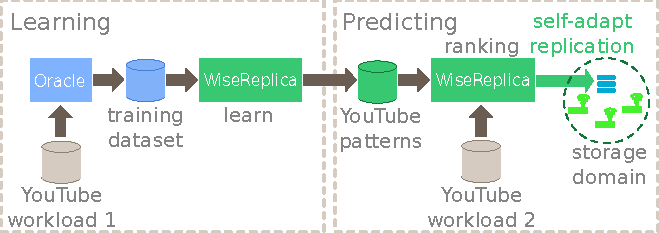
\includegraphics[width=.65\textwidth]{inputs/img/wisereplica_scheme}
  \caption{Framework for learning and predicting ranking of Internet videos .}
  \label{fig:model_scenario}
\end{figure}

\section{Boosting VoD delivery: The WiseReplica Approach}
\label{sec:replication_scheme}

In this section, we describe WiseReplica replication scheme. First, we highlight how WiseReplica operates in edge networks, by in introducing the concept of storage domains. Then, we explain its replication strategy based on predictions of ranking of video demand.

\subsection{Distributing VoD with Storage Domains}
\label{subsec:replication_scheme_sd}

% We evaluated this work with an implementation on top of PeerSim. We developed a tool which models a content distribution system for edge networks. 

We assume that WiseReplica operates in peer-assisted VoD systems deployed on hybrid CDN platforms. We consider the hybrid CDN design called Caju, that is detailed in our previous work~\cite{caju_tr_2012} as our target platform. It is based on sets of devices located close to customers, named storage domain. A storage domain is a logical
entity that combines resources from both datacenters and edge networks in the last mile of the content delivery chain. As Figure~\ref{fig:storage_domain} shows, devices in a storage domain can play either a coordinator or peer role. 

\noindent
\textbf{Coordinator} is a server or a small-sized cluster of servers deployed in the nearby datacenter. We assume that the coordinator performs scheduling of video requests for the local storage domains. Therefore, it runs the main instance of WiseReplica, and keeps information about resources consumption. Its main goal is to maintain the right number of replicas per video in the local peers, by pre-fetching or deleting sources. Instead of always contacting the content providers, coordinators might interoperate in logically centralized way to fetch videos that have been vanished from a storage domain. They store the most recent videos in their own cache for replication purposes. Whenever a new replica is necessary, the coordinator pushes it to a randomly, uniformly selected peer. Similarly, coordinators send video deletion requests to local peers. 

\noindent
\textbf{Peers} is a set of devices located close to each other through which customers get network access, e.g. home gateways connected to the same digital subscriber line access multiplexer (DSLAM). These devices actually deliver videos to customers in a storage domain, being the main source of storage and network resources. They execute scheduling and replication commands sent by the storage domain's coordinator. Each peer contributes with a percentage of storage and network resources to the system, as in a collaborative caching. In the local cache is applied the LRU policy for videos replacement.

This model is specially interesting for the problem of videos delivery as it takes advantage of nodes geographical position~\cite{Brodersen_www_2012}. It provides two main infrastructure properties to WiseReplica: replication group and hop limit.  The replication group allows WiseReplica to adapt video replication for smaller sets of peers, most likely connecting customers with similar content interests. By enforcing a hop limit, storage domains avoid jitter, ensure low latencies, and permit WiseReplica improving  the efficiency of network resource provision. 

In addition, we assume that a storage domain enforces an initial placement policy. This policy defines the minimum replication degree $m$ for initial copies for any new, just fetched Internet video.  Request scheduling is simple. A view request is served by at most $R$ nodes with uniform load. Available sources come from $r=min(n,R)$, where $n$ is the number of current replicas. In this work, we consider $m$ equals to two and $R$ equals to five as default settings. For requests scheduling, this approach enforces well-known policies for peers in edge networks, including nearest source selection and multi-sourcing. 


\begin{figure}[htbp]
  \centering
  \begin{minipage}[t]{1\linewidth}
    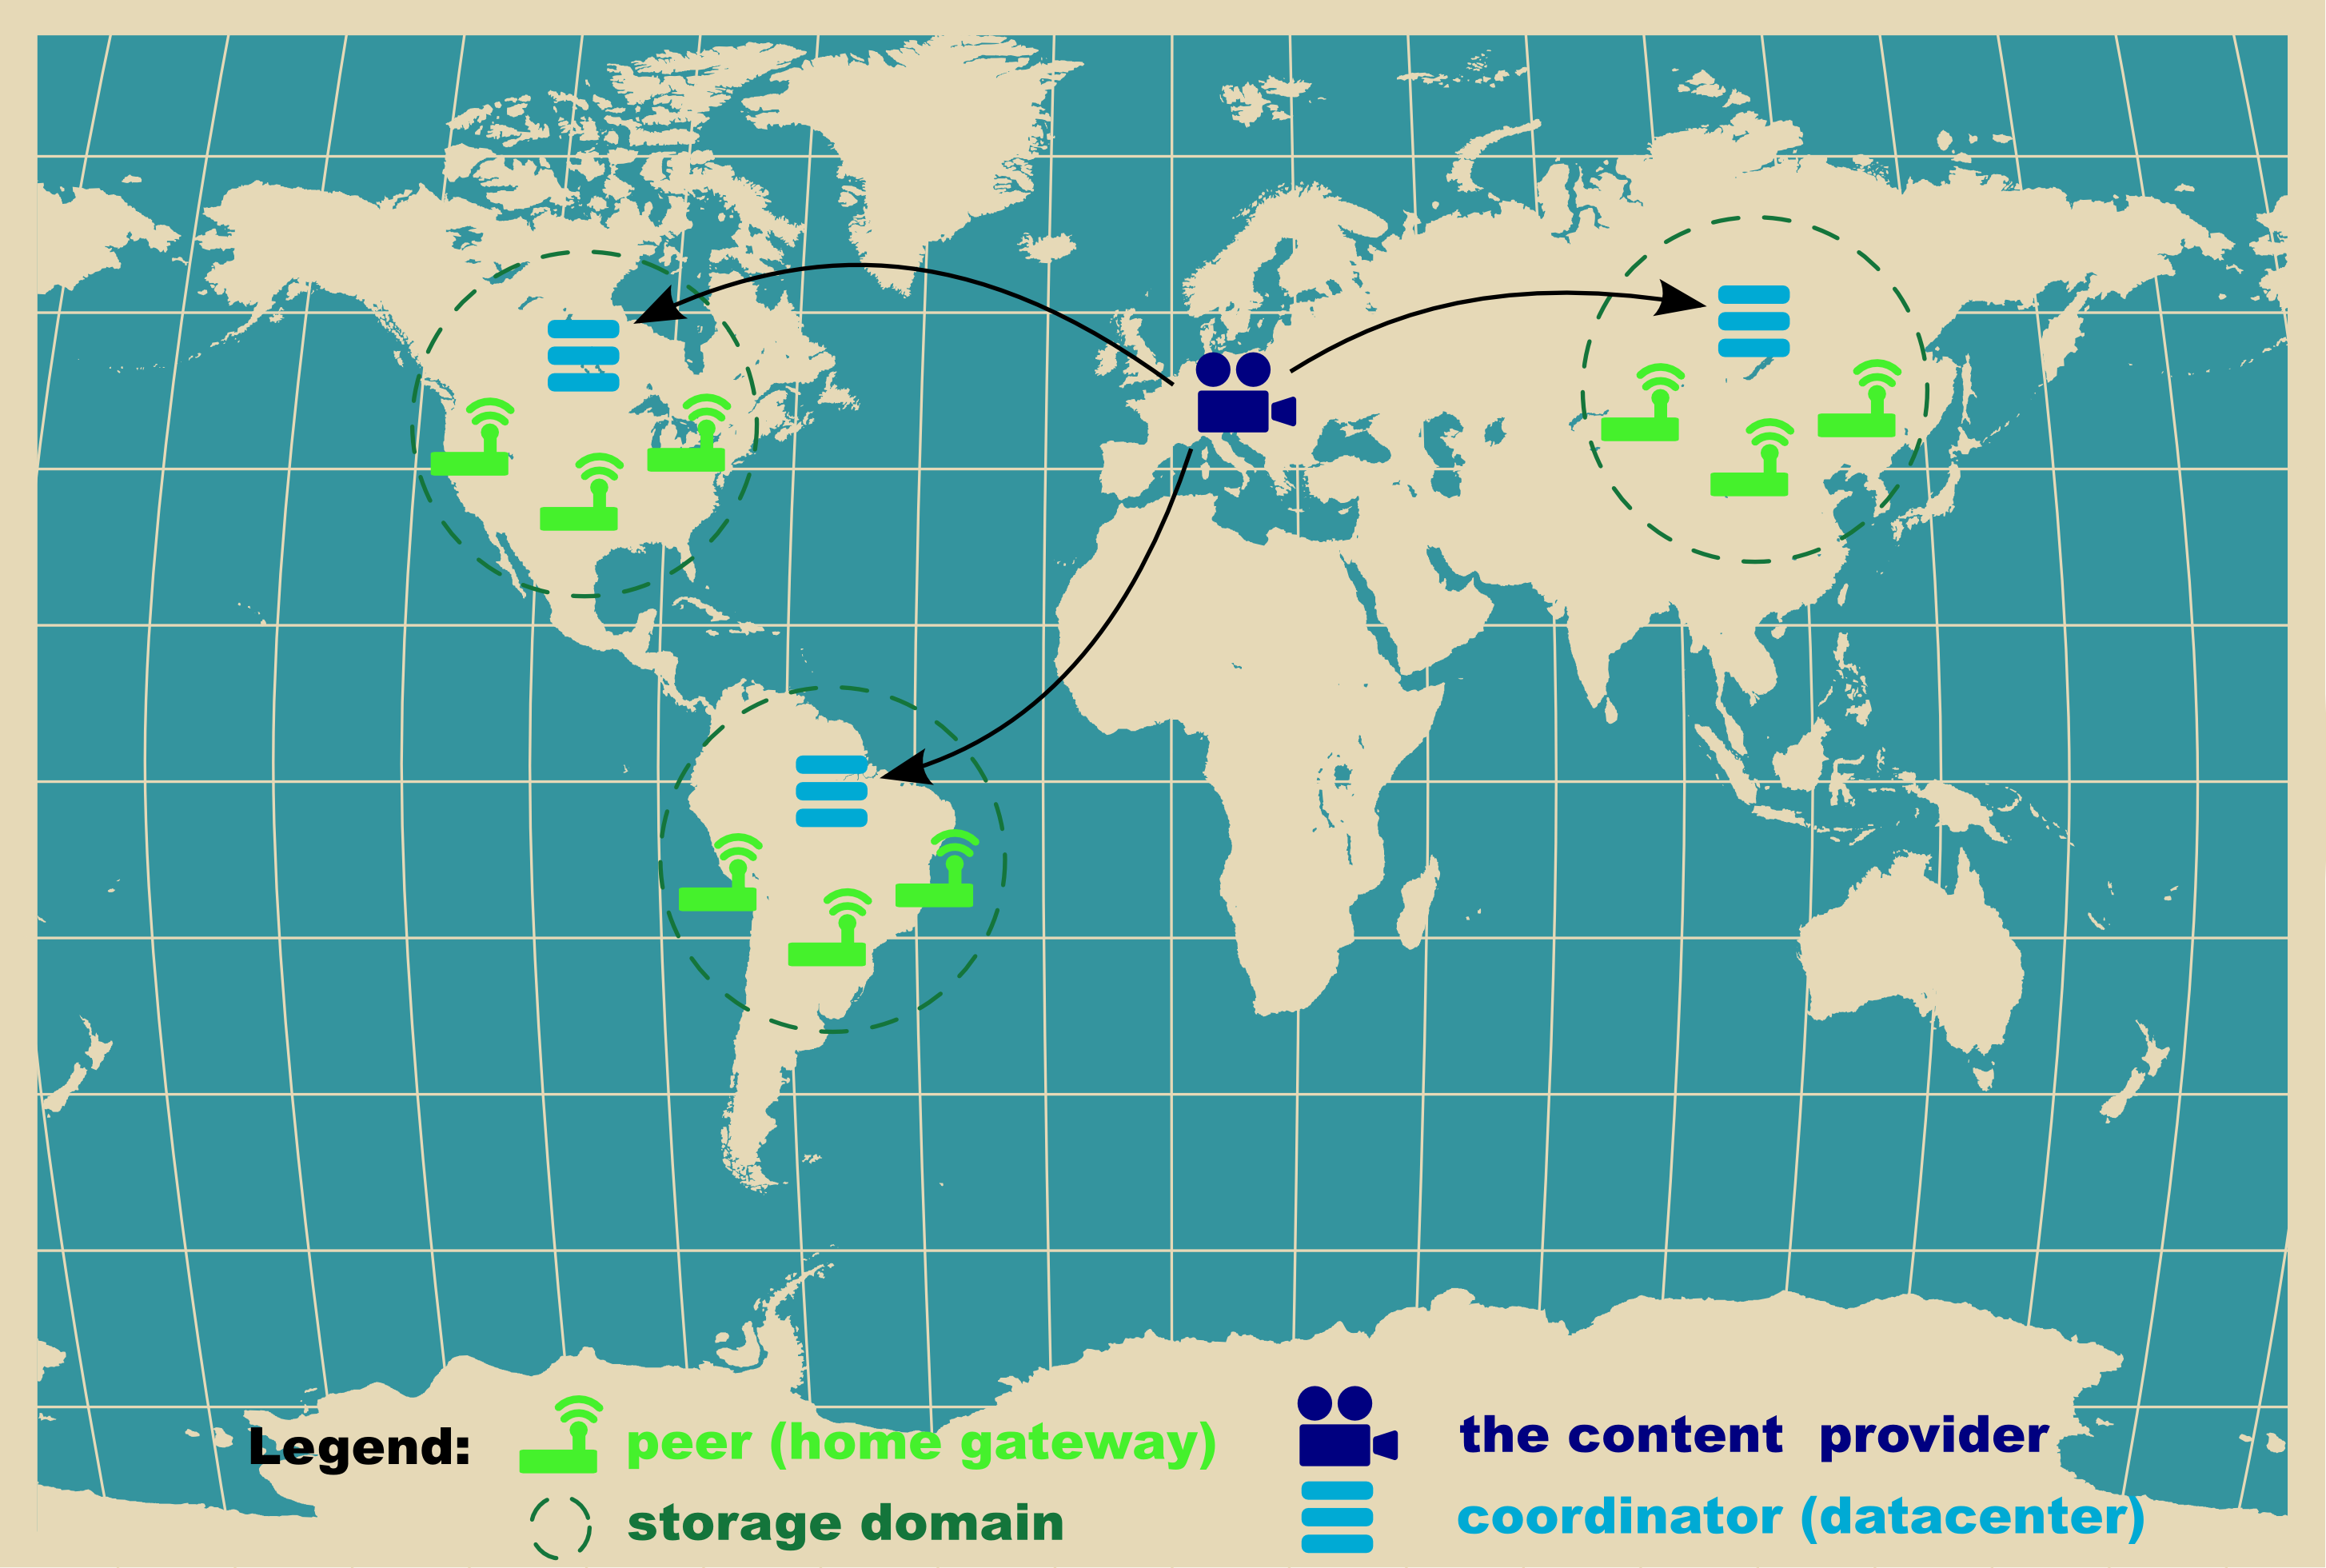
\includegraphics[width=1\textwidth]{inputs/img/sd}
    \caption{Storage domains.}
    \label{fig:storage_domain}
  \end{minipage}
\end{figure}

%We assume that the service provider infrastructure is organized in
%federated storage domains. A storage domain is a logical entity that
%aggregates a set of storage elements that are located close to each
%other, e.g. connected to a digital subscriber line access multiplexer
%(DSLAM). The storage elements are partitioned in two different
%classes: (i) operator-edge elements, furnished by storage operators,
%e.g. small-sized datacenters, and (ii) consumer-edge entities provided by
%consumers, such as set-top boxes. Consumer-edge devices contribute to
%storage and network resources according to their availability and
%load. Operator-edge nodes run a distributed storage system for local-area
%network over commodity servers. They provide cheap and high available
%resources dedicated to the storage service.
%
%On top of each Storage Domain runs a couple of services that deals with
%serving clients' requests, and performs appropriate object data
%placement and replication. 



\subsection{Self-adapting Replication According to the Ranking of Internet Videos}
\label{subsec:wisereplica_replication_strategy}

Our utmost goal is to contribute to meet increasing customers expectation on Internet videos using peer-assisted VoD systems. To enhance VoD delivery, we assume that rebuffering is a major issue to be addressed. We propose to cope with this issue by enforcing minimum average bitrate of each streaming as the main QoS metric. In this scenario, content and CDN providers must be committed to enforce minimum average bitrate for videos through SLA contracts. Since Internet videos delivery is a resource-hungry service, we must also adapt the network provision and storage usage as we aim to prevent violations. To this end, we propose WiseReplica, an adaptive replication scheme for peer-assisted VoD systems based on storage domains.

WiseReplica maintains replicas inside a storage domain. Running on the coordinator, it adapts the replication degree of Internet videos of a storage domain according to a machine-learned ranking. Our scheme follows a three-part procedure: 

\noindent
\textbf{Collect information from the request arrival process}. For each video request, WiseReplica collects 10 lightweight measurements. The goal is to gather comprehensive information for measuring the video demand and accurately predicting the raking. As described in Section~\ref{sec:learning_model}, they are video size, network availability, network usage (load), current number of viewers and replicas, inter-arrival time between requests (delta), aggregate number of views, mean of time between requests (mtbr), life time, and average bitrate. We compute averages and means from the last up to five requests. It is important to notice that all these measurements can be easily collected in the storage domain's coordinator.
 
\noindent
\textbf{Rank Internet videos in order of demand}. Based on the measurements of the request arrival process, we use the learning model described in Section~\ref{sec:learning_model} for predicting the rank position of Internet videos demand. We can predict the video rank for each view from the second request. The ranking comprises information about demand and QoS requirements. Predictions are quite essential for enhancing VoD delivery. Since our learning model make predictions on a request basis, WiseReplica can react to the video demand as promptly as the rank position evolves. Indeed, ranking is an intuitive way to capture the demand of videos in peer-assisted VoD systems. The higher is the demand rank position of an Internet video, the higher is the demand for it. There are four positions on our machine-learned ranking: \emph{non-popular, popular, very popular,} and \emph{viral}. WiseReplica has a straightforward strategy to perform replication according to hotness rank positions. Videos that fall into the lowest rank position can have their replication degree reduced, otherwise they need more replicas. Thus, the maintenance of replication degree of Internet video, including video creations and deletions in peers, relies on replication policies.

\noindent
\textbf{Enforce replication policy accordingly and in time}. The goal of replication policies is two-fold: first (i) ensure consumers' expectations in time and (ii) reduce the total number of replicas as much as possible. For that, WiseReplica must adapt replication of videos according to the forecasts of their rank positions. Our replication scheme enforces two types of replica maintenance policies: deletion and creation policy. In this work, we enforce a single video deletion policy.  Whenever the coordinator receives a request to a video in the non-popular rank, the deletion policy says that one replica is deleted until the minimum replication degree $m$ is reached. Similarly, our scheme periodically runs a maintenance procedure (e.g. each five minutes) to smoothly enforce the deletion policy for inactive videos. This allows WiseReplica to reduce the total number of replicas. To cope with SLA violations and meet customers' expectations, we evaluate four quite simple policies, namely uniform, linear, quadratic, and exponential. They are respectively defined as follows: $B$, $Br$,$Br^2$, and $B^r$, where $B$ is a constant that represents the target number of replicas, and $r \in \{1,2,3\}$ the rank positions. We report on creation policies' performances in Section~\ref{sec:evaluation}.


Our findings show that this approach produces a good balance between resource usage and consumers' satisfaction. It is important to note, however, WideReplica does not cover video durability, neither does fault-tolerant mechanisms (e.g. failure detection/recovery procedures). Rather, our goal is to improve VoD availability, boosting network provision, meeting consumers' expectations on VoD services, and reducing storage usage as much as possible. To this end, WiseReplica combines lightweight measurements, accurate predictions of Internet videos ranking, and replication policies enforcement in a particularly novel, flexible way. In peer-assisted VoD systems, it can easily interoperate with de facto approaches, including HTTP adaptive streaming technique and swarming protocols, such as BitTorrent. 

\section{Simulation Methodology}
\label{sec:simulation_methodology}

We simulate a peer-assisted VoD system based on a hybrid CDN design called Caju~\cite{caju_tr_2012}. We evaluate WiseReplica using YouTube traces. We compare WiseReplica performance with other two adaptive replication schemes, namely non-collaborative caching and Oracle-like collaborative caching. The aim of our simulations is to study in details the variability of demand and resource allocation of VoD services on edge networks, and the performance of replication schemes in enforcing expected Internet video availability.

\subsection{Workload from YouTube Traces and SLA definition}
\label{subsec:methodology_workload}

The workload and SLA definitions are at the core of our evaluation. We define a workload that captures the main features of VoD services using YouTube traces, and a SLA contract that meets users' expectations. 
 
In the workload definition, we are particularly interested in reproduce a realist request arrival process, placing the emphasis on popularity growth and video encodings. Thus, we use YouTube traces, presented in Subsection~\ref{subsec:motivation_youtube_traces}. Before integrating YouTube traces to our workload, we first preprocessed their YouTube datasets to remove inconsistent measurements, such as videos with no views. Basically, we got rid of videos with small number of total views (those smaller than the first quartile) and videos with few daily measurements (those smaller than the third quartile). That allowed us to pick off 20\% most representative YouTube growth patterns, accounting for 21827 distinct curves. Then, we randomly selected, with a uniform distribution, curves from this preprocessed data to be assigned to videos of our workload. Similarly, we assigned high quality YoutTube video encodings  to our workload videos, based on advanced settings depicted in Table~\ref{tab:youtube_encodings}. To summarize, Table~\ref{tab:workload_parameters} lists default values for workload parameters. Finally, videos are always divided and distributed in chunks or segments of fixed size, 2MB.

\begin{table}
  \label{tab:workload_default_parameters}
	\begin{center}
		\caption{Default values for workload parameters.}
  		\label{tab:workload_parameters}
		\begin{tabular}{|p{6cm}|p{6cm}|l|}
			\hline
			\multicolumn{2}{|c|}{Workload} \\
			\hline
			\hline
			Requests per user&uniform\\
			\hline
			Experiment duration&4 hours\\
			\hline
			Mean requests per second&100\\
			\hline
			Requests fractions&5\% of creations, 95\% of views\\
			\hline
			Video size (follows Pareto)&shape=3,between 13MB and 1.6GB\\%\\
			\hline
			Video popularity (Zipf-Mandelbrot)&shape=0.8, cutoff=number of videos\\
			\hline
			Videos{'} creation (Poisson)&$\lambda$=creations per second\\
			\hline
			Popularity growth from YouTube traces&21827 distinct patterns\\
			\hline
			YouTube encoding settings (bitrates)&5Mbps, 15Mbps, 30Mbps, 50Mbps\\
			\hline
		\end{tabular}
	\end{center}
\end{table}

In terms of SLA definition, we assume that content and content delivery providers are committed to improving the Internet video availability for customers in a content-oriented approach. In our case, a good peer-assisted VoD system must ensure videos availability by avoiding rebuffering. Therefore, we consider a global, simple SLA contract drawn up to provide a minimal average bitrate according to each Internet video encoding setting. A SLA violation happens whenever the system fails to enforce the minimal average bitrate for any viewer's request. 


\subsection{Evaluation Scenario}
\label{subsec:methodology_evaluation_scenario}

\begin{figure}
  \centering
     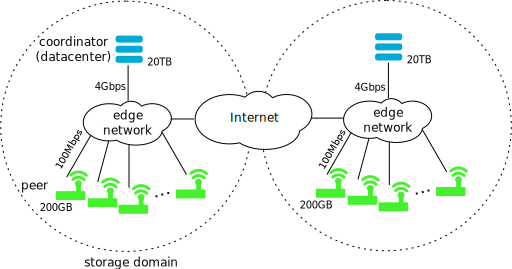
\includegraphics[width=.9\textwidth]{inputs/img/evaluation_scheme}
  \caption{Evaluation scenario.}
  \label{fig:evaluation_scenario}
\end{figure}

Our evaluation scenario (Figure~\ref{fig:evaluation_scenario}) includes 4002 nodes, arranged across two storage domains. There are one coordinator and 2000 peers per storage domain. Storage and network capacities differ according to the device role. Coordinators have 20TB of storage capacity and full-duplex access link of 4Gbps. Peers contribute 200GB each, equipped with 100Mbps full-duplex links. Note that the two coordinators contribute with a small fraction of aggregate edge resources, i.e. 5\% of the storage capacity and only 2\% of the total network capacity. This draws our attention to the performance of replication schemes towards peers resource allocation. We assume only 1\% peers' storage is available for caching additional replicas, namely 2GB.

We implemented and evaluate this work using simulation. To this end, we developed a simulation tool on top of PeerSim~\cite{p2p09-peersim} to implement storage domains in edge network and bandwidth scheduling.Our design focus on network's resource allocation accuracy for simulating bitrate enforcement and concurrent videos views properly.  Design and implementations details of our tools to simulate network resource scheduling are available in our previous work~\cite{silvestre2010most}. We have performed our simulations using servers equipped with Intel Xeon E5450 3.00 GHz, and a RAM of 4GB. 

\subsection{Comparable Replication Schemes}
\label{subsec:methodology_replication_schemes}

We compare WiseReplica with two other schemes.

\noindent
{\bf Non-collaborative caching}. Adaptive replication schemes based on non-collaborative caching, such as those that uses Least Recent Used (LRU) algorithm, are easy to implement and deploy. A new replica is created in a peer whenever a user requests to view a video. LRU replacement is enforced regarding the static percentage of the local storage capacity for caching of 1\%.

\noindent
{\bf Oracle-like collaborative caching}. This is an idealized benchmark case. Here, we assume a peer-assisted VoD system deployed in a network that runs a deadline-aware transport protocol, similar to Wilson \emph{et al.}\cite{d3_sigcomm2011} work. Based on our previous work with AREN~\cite{silvestre_aren_icpads12}, an adaptive replication scheme for edge networks, we implemented a benchmark replication scheme that relies on bandwidth reservation and collaborative
caching to provide an adaptive number of replicas for videos. We replicate videos according to aggregate network usage by enforcing a low and high thresholds. This makes the video replication a function of bandwidth reservation, and ensures that network and storage provision follows video demand properly, as depicted in Figure~\ref{fig:oracle_like}. Per video, we consider two percentage thresholds for aggregate network usage: $P_{min}$ and $P_{max}$. Our replication strategy works as follows. A video $v$ that has $N$ replicas in peers with network capacity of $b$ requires more replicas if the current bandwidth reservation $U(v) > P_{max} \sum_{i=1}^N b$. Similarly, if $U(v) < P_{min} \sum_{i=1}^N b$, replicas can be deleted. Otherwise, keep the replication degree. Although this empirical approach is hard to be adopted in a real deployment, our previous results~\cite{silvestre_aren_icpads12} suggest that it allows us to achieve near-optimal results, preventing \emph{all} SLA violations, enhancing network usage and decreasing storage usage dramatically.  

\begin{figure}
  \centering
     
\includegraphics[width=.6\textwidth]{inputs/img/oracle_like}
  \caption{Oracle-like bandwidth management for a video, illustrating aggregate bandwidth for $N$ replicas and $b$ available bandwidth, bandwidth reservation (bandwidth usage) and thresholds ($P_{min}$ and $P_{max}$).}
  \label{fig:oracle_like}
\end{figure}


\subsection{Collecting the Datasets for Learning}
\label{subsec:methodology_training_dataset}

To perform rank predictions of Internet videos, we need training datasets from which we can learn the behaviour of video demand in peer-assisted VoD systems. In this section, we explain the methodology for gathering data for these predictions. 

The training dataset of our prediction model comes from measurements of the request arrival process on per-assisted VoD systems, as described in Subsection~\ref{subsec:learning_model_details}. Each line of our training dataset has 11 values, 10 input measurements about a video current state, and, as a label, that represents rank position. Although, the datasets evaluated in this work were synthetically collected by performing simulations with the Oracle-like benchmark replication approach (detailed in Subsection~\ref{subsec:methodology_replication_schemes}), similar datasets can be collected from monitoring systems of running CDN systems.

In this work, Oracle-like benchmark replication approach (Subsection~\ref{subsec:methodology_replication_schemes}) represents the near-optimal way to serve VoD service according to video encodings and popularity, whose functioning we are very interested in learning. In this empirical approach, a video requires additional replicas only if there exists a certain number of concurrent accesses, where concurrence is measured by checking a high threshold of the current reserved bandwidth, as detailed in Subsection~\ref{subsec:methodology_replication_schemes}. We assume that popular videos are those that have additional replicas during its lifetime. Since Internet videos popularity distribution follows a Zipf-like distribution~\cite{popularity_prediction_2010}, concurrent access are rare events as well as popular videos classified by this approach, thus it provides a quite fair approach to identify popular videos. 

Raw data from Oracle-like technique permits easily distinguishing between two ranking positions only, non-popular and popular videos, i.e. requests to non-popular videos are all those that do not trigger any replica creation, or those that resulted in deletions. However, there is a lack of information about different ranking positions of popular videos. Hence, depending on the frequency of replica creation, we add information to requests to popular videos classifying them in popular, very popular, or viral. To define these three levels of \emph{hotness}, we run simulations with YouTube traces, collected the distribution of replicas creation in milliseconds, and split it in three nearly equal parts by observing the 66-percentile and 33-percentile inter-creation time for new replicas. This means that the higher is the frequency of replica creation, the hotter is the video, and the higher is the ranking position. Now, collected data suit model's definitions very well. 

\section{Evaluation}
\label{sec:evaluation}

The utmost goal of our performance evaluation is two-fold: (i) measure the accuracy of our learning model in ranking Internet videos in order of \emph{hotness}, and (ii) evaluate the performance of our replication scheme in meeting viewers' expectations in peer-assisted VoD systems. Further details about evaluation set-up are available in Section~\ref{sec:simulation_methodology}.

\subsection{Performance Evaluation Metrics}
\label{subsec:methodology_metrics}

We aim to evaluate the performance of two main WiseReplica modules: machine-learned ranking and replication strategy. Hence we group evaluation metrics as follows:

\subsubsection{Machine-Learned Ranking Accuracy.} 

\ We adopt the normalized Discounted Cumulative Gain (nDCG) criterion as the main evaluation metric for our learning model. nDCG is a standard quality measure in information retrieval, especially for Web search~\cite{jarvelin2002cumulated}. The DCG definition is $DCG_{L}=\sum_{i=1}^L \frac{2^{F(i)}-1}{\log_{2}(1+i)}$, where $L$ is the global set of ranked videos, and $F(i)$ is the rank position of $i$th video. To compute nDCG, we divide DCG measure by the idealized DCG with perfect order of the set $L$. Thus, the perfect model scores $1$. Unlike typical information retrieval problems, as a ranking of web content, our model does not have the notion of \emph{query}. Instead, we rely on nDCG robustness to measure the performance of our learning model as a global ranking problem. Since the ranking problem shares properties with both classification and regression problems, we compare nDCG to other three popular machine learning metrics: the mean square error, a standard metric for regressions; precision, for classification; and a less robust, well-known variant of nDCG, namely  in this work nDCG(2). We evaluate three different state-of-the-art ensemble learning methods available in \textsc{Scikit-learn} library: \textsc{Random Forest}, \textsc{Extremely Randomized Trees}, and \textsc{Gradient Tree Boosting}. Moreover, we report briefly on the sample size for learning, number of estimators or learners of ensemble methods, measurements or features importance, and the computational overhead of our model, including memory usage and computation time for prediction.

\subsubsection{Metrics for Replication Strategies in Peer-Assisted VoD Systems.} 

\ Assuming that content and CDN providers are committed to enforcing bitrate as main QoS metric through SLA contracts, we consider SLA violation as the primary performance metric. Thus, a SLA violation happens whenever the peer-assisted VoD system does not provide the minimum average bitrate for preventing rebuffering. This measures the WiseReplica capacity of meeting consumers' expectations. We also investigate the impact of our replication scheme using storage domains in peer-assisted VoD systems. To this end, our evaluation metrics are network and storage usage. Finally, we compare WiseReplica results with a non-collaborative caching and the Oracle-like assumption, described in Subsection~\ref{subsec:methodology_replication_schemes}. 

\subsection{Fitting and Measuring the Accuracy of Our Ranking Model}
\label{subsec:prediction_performance}

The evaluation of our learning model comprises: ensemble method selection, number of \emph{estimators},  sample size for leaning, and inputs' relative importance. In this subsection, we aim to evaluate the most important settings and tune our model towards higher accuracy, using the learning framework described in Subsection~\ref{subsec:framework}.

\subsubsection{Selecting and Fitting an Ensemble Method.}

\ Ensemble methods have become very popular in statistical learning. Their algorithms combine several \emph{estimators} or \emph{week learners} to provide robust learning models and prevent overfitting. We fit and evaluate our model with three methods from \textsc{Scikit-learn} library: \textsc{Random Forest}(RF), \textsc{Extremely Randomized Trees}(ET), and \textsc{Gradient Tree Boosting}(GB). We consider two distinct samples with 124 thousand lines each, one for training and other for testing. We set to 10 the number of estimators as a common setting. All other parameters have default settings. Based on four metrics detailed on Subsection~\ref{subsec:methodology_metrics}, \textsc{Random Forest} fits our model better. Figure~\ref{fig:ensemble_method_eval} depicts three of these metrics. \textsc{Random Forest} performs particularly well in nDCG score, the main metric for ranking problems. While \textsc{Extremely Randomized Trees} and \textsc{Gradient Tree Boosting} score 0.9126 and 0.4128 respectively, \textsc{Random Forest} scores 0.9594. In terms of precision, \textsc{Random Forest} slightly better, with a score of 0.9922.  \textsc{Extremely Randomized Trees} scores 0.9899, and \textsc{Gradient Tree Boosting} scores 0.9502.  It also outperforms the other two methods regarding the mean square error metric, scoring 0.0094 compared to 0.0122 with \textsc{Extremely Randomized Trees} and 0.1021 with \textsc{Gradient Tree Boosting}. nDCG(2) metric confirms these results. Therefore, we select \textsc{Random Forest} method for implementing our prediction model and nDCG as the key accuracy metric for ranking predictions. 

\begin{figure}[htbp]
	\begin{minipage}[t]{0.48\linewidth}
     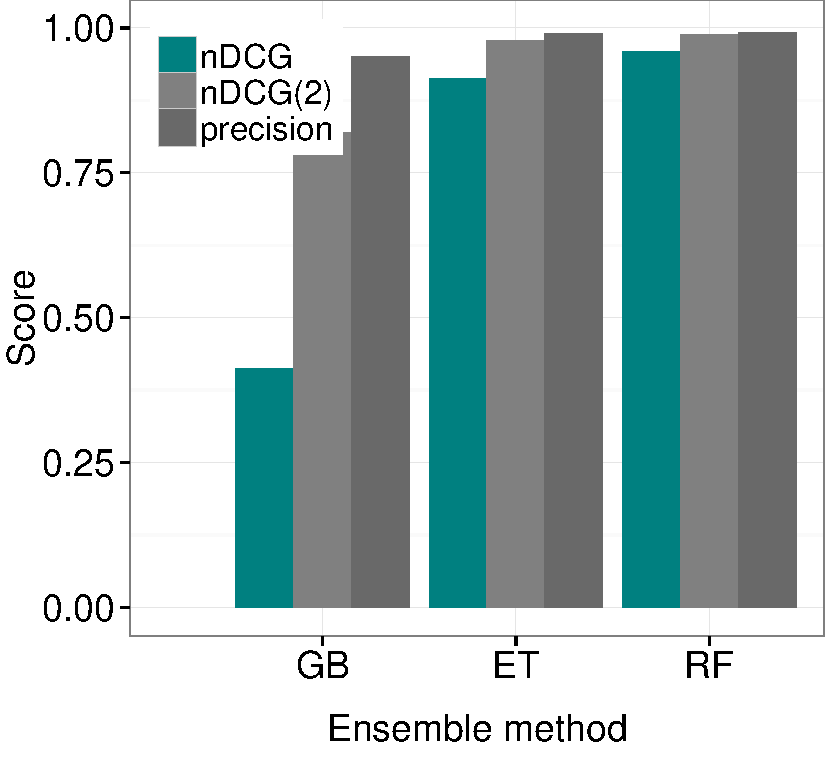
\includegraphics[width=.95\textwidth]{inputs/img/ensemble_method_eval}
		\caption{Ensemble methods evaluation: \textsc{Random Forest}(RF), \textsc{Gradient Tree Boosting}(GB) and \textsc{Extremely Randomized Trees}(ET).}
		\label{fig:ensemble_method_eval}
  %\centering
	\end{minipage}
	\hspace{0.1cm}
	\begin{minipage}[t]{0.48\linewidth}
		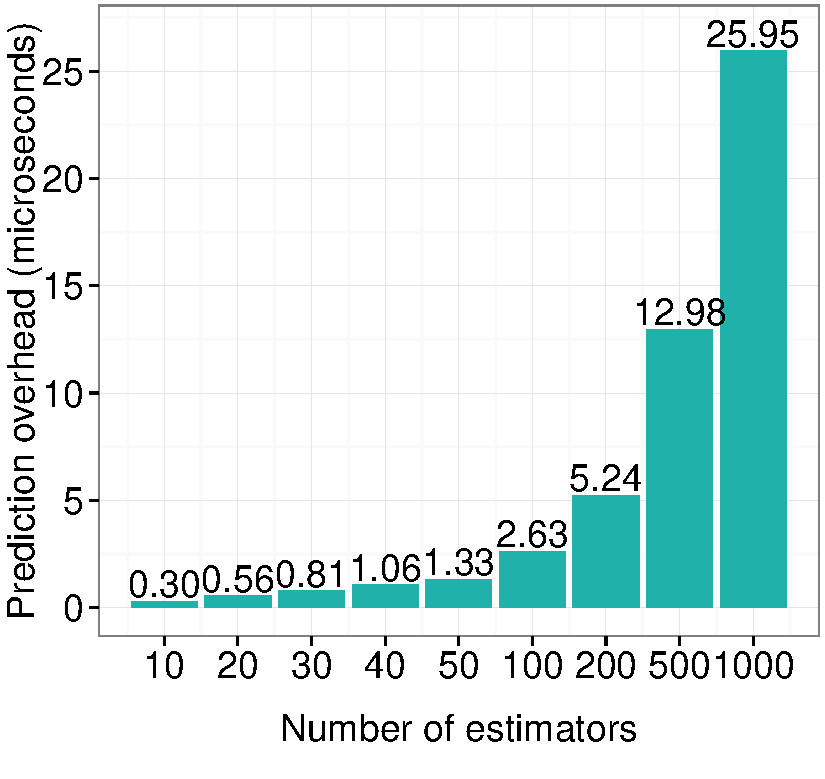
\includegraphics[width=.95\textwidth]{inputs/img/rf_learners}
		\caption{Overhead for different number of estimators of \textsc{Random Forest}.}
		\label{fig:rf_learners}
	\end{minipage}
\end{figure}

\subsubsection{Adjusting the Number of \emph{Estimators} to Learn.}

\ According to Friedman \emph{et al.}, \textsc{Random Forest} performs predictions by building a collection of \emph{de-correlated} trees, namely estimators, and then averages them. We investigated the impact of the number of estimators in ranking accuracy, memory and computation time. We varied the number of estimators progressively from 10 to 1000, with the same previous samples. Results show that the number of estimators has a negligible impact in the accuracy of our model. While a model with 10 estimators scores 0.9594, 1000 scores 0.9569, slightly worse. One reason for this might be the number of inputs, relatively small, that is likely to require a small number of estimators. Yet, the number of estimators impacts on the model overhead, specially for computation time. As depicted in Figure~\ref{fig:rf_learners}, the computation time ranges from 0.3 microseconds with 10 estimators to almost 26 microseconds with 1000 ones. Although the worst case still represents low overhead, the lower the better. Memory overhead is rather negligible, ranging from 30 to 32MB. Overall, our model has a quite low overhead, suitable for going online in large peer-assisted VoD systems. Since there is no evidence to increase the number of estimators, we keep 10 estimators as a default, fair setting.

\subsubsection{Evaluating Bigger Samples for Fitting the Model.}

\ Towards a higher accuracy, we evaluated bigger samples for fitting our prediction model in its learning phase, described described in Subsection~\ref{subsec:framework}. We collected more information by running logger simulations. As expected, Figure~\ref{fig:sample_size} confirms that we improve accuracy through bigger samples. The improvement in accuracy was slight, about 0.03 as we use a sample size almost six times bigger, i.e. 683 thousand. It is quite important to highlight, though, that this has no impact on computation time of predictions. Thus, we use the biggest sample for the remaining evaluations.

\begin{figure}[htbp]
	\begin{minipage}[t]{0.48\linewidth}
     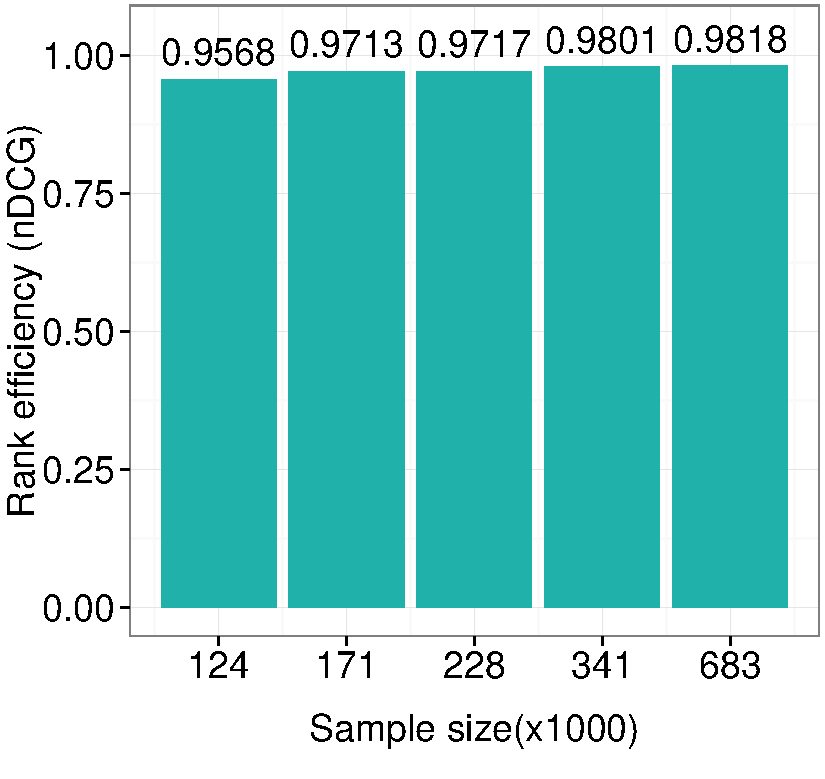
\includegraphics[width=.95\textwidth]{inputs/img/sample_size}
		\caption{Accuracy with different sample sizes.}
		\label{fig:sample_size}
  %\centering
	\end{minipage}
	\hspace{0.1cm}
	\begin{minipage}[t]{0.48\linewidth}
		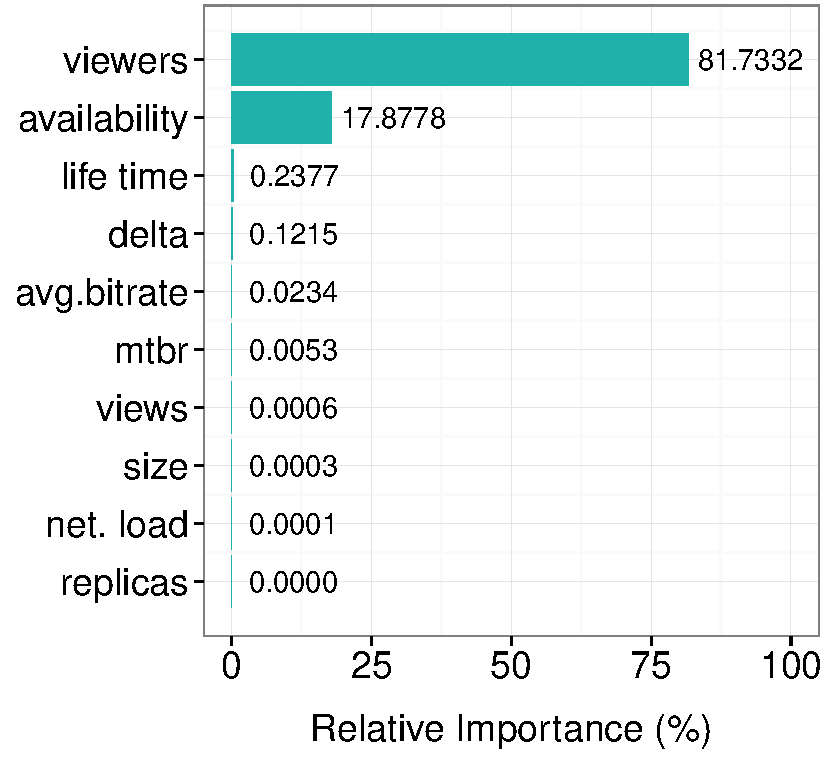
\includegraphics[width=.95\textwidth]{inputs/img/feature_importance}
		\caption{Relative importance to ranking of the 10 model's inputs.}
		\label{fig:feature_importance}
	\end{minipage}
\end{figure}

\subsubsection{Analysing the Relative Importance of Model's Inputs.}

\ We were particularly interested in evaluating the contribution of each input of our model, described in Subsection~\ref{subsec:learning_model_details}. \textsc{Scikit-learn} library allows us to measure the relative importance of each input for predicting the ranking position using the \textsc{Random Forest} method. Figure~\ref{fig:feature_importance} highlights the relative importance for all 10 inputs of our ranking model. The two most relevant inputs are the current number of viewers and network availability. These inputs alone account for 99.6\% of the all model's accuracy. It seems quite reasonable, since the former measures the demand for a video and the later depicts the offer of network resources, the main system feature for enforcing average bitrate. Based on the analysis of the current datasets, the remaining eight inputs are less important to the ranking model's accuracy. Surprisingly, the number of replicas, current network load, and video size seem to be useless to our model. It is likely that network availability is a particularly good measurement, making these eight inputs rather redundant. For simplicity, we include all inputs in the rest of the work. This is harmless for the model's accuracy.

\subsection{Evaluating Replication Strategies in Peer-Assisted VoD Systems}
\label{subsec:performance_evaluation}

In this subsection we analyse the replication strategy used in WiseReplica. First, we evaluate four simple replication policies. Then, we compare WiseReplica with a non-collaborative caching and Oracle-like benchmark replication approach, both described in Subsection~\ref{subsec:methodology_replication_schemes}. We evaluate their capacity to meet consumers' expectation by observing the number of violations. In addition, we compare their resource allocation performance regarding network and storage usage.

\subsubsection{Enforcing Simple Replication Policies on Ranked VoD}

For the three highest rank position, WiseReplica enforces a replica creation policy, described in Subsection~\ref{subsec:wisereplica_replication_strategy}. It defines the replication degree growth factor. Considering the smallest evaluated system load (with mean video size of 20MB), we analyse four simple creation policies, namely uniform, linear, quadratic, and exponential.  Table~\ref{tab:creation_policies} shows the number of violations by varying $B$ from 2 to 6. Overall, creation policies that take into account the rank positions, i.e. linear, quadratic, and exponential, performed better. Results show that there is relatively small difference for $B\ge 3$, suggesting that our ranking model reacts promptly to modifications on network availability, preventing over-replication. However, for $B\ge 5$, it appears that replication increases the network load system load, causing few more violations. We selected the linear policy with $B=4$ that seems to be the most resilient towards proper resource allocation, providing a fair replication degree growth factor.

\begin{table}
  \label{tab:motivation_advanced_encodings}
	\begin{center}
		\caption{Replication policies.}
  		\label{tab:creation_policies}
		\begin{tabular}{p{2cm} || p{1cm} p{1cm} p{1cm} p{1cm} p{1cm}}
		%\begin{tabular}{r||r r r r}
			&\multicolumn{5}{c}{{\bf Parameter $c$}}\\
			{\bf Policy}&{\bf 2}&{\bf 3}&{\bf 4}&{\bf 5}&{\bf 6}\\
			\hline
			\hline
			Uniform&867&567&\cellcolor{blue!25}44&28&23\\
			\cellcolor{blue!25}Linear&\cellcolor{blue!25}123&\cellcolor{blue!25}77&\cellcolor{blue!25}6&\cellcolor{blue!25}9&\cellcolor{blue!25}16\\
			Quadratic&102&21&\cellcolor{blue!25}42&46&58\\
			Exponential&118&32&\cellcolor{blue!25}19&27&28\\
		\end{tabular}
	\end{center}
\end{table}

\subsubsection{Load Resiliency.}

\ A good replication strategy must cope with changes on the system load.  We vary the global load of the system by changing the mean video size, described in Subsection~\ref{subsec:methodology_workload}. Assuming the three mean video sizes, namely 20MB, 30MB and 40MB, caching had 1814, 3864, and 7049 violations respectively, while WiseReplica had only 6, 77, and 106. Figure~\ref{fig:mean_load_bar} compares the number of violations using WiseReplica and a non-collaborative caching. As the load of the system increases, concurrency in bitrate allocation also increases, causing more violations. WiseReplica outperforms caching mostly because it predicts and prevents useless replication. Therefore, we set to the highest evaluated system load, 40MB, as the default mean video size workload setting.

\begin{figure}
  \centering
     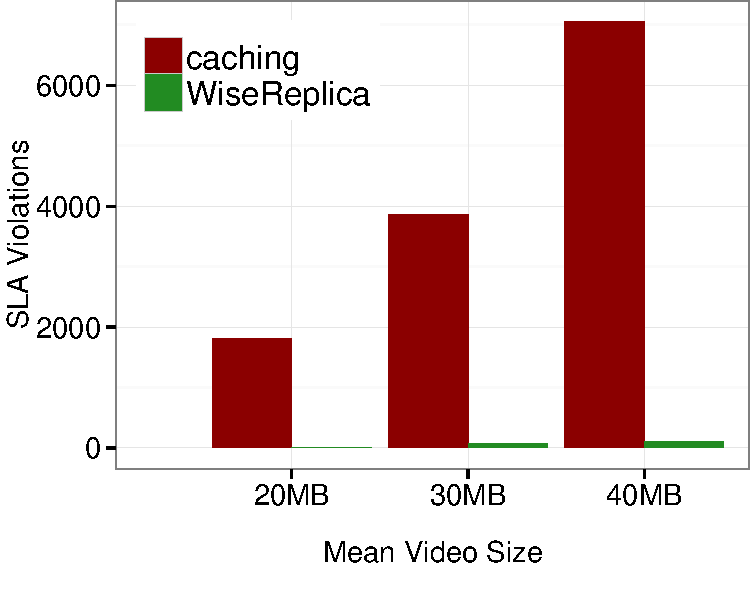
\includegraphics[width=.6\textwidth]{inputs/img/mean_load_bar}
  \caption{Mean Video Size. Higher loads increase the concurrence in network resources, as a result, more violations.}
  \label{fig:mean_load_bar}
\end{figure}

\subsubsection{Benefits of Prediction on Storage Usage.}

\ We aim to adapt the number of replicas to the number of views of a video, especially for the most popular ones. Figure~\ref{fig:replication_for_most_popular} plots the maximum number of replicas for the 1\% most popular videos. Using caching, the maximum number of replicas is high, ranging from 816 to 1367. The Oracle-like assumption allows to decrease significantly the lower and upper limits, to 10 and 190. WiseReplica also reduces the maximum replica range, which is from 19 to 160. More interestingly, the shape of the replication curves of WiseReplica and Oracle-like are quite similar indeed. It confirms that our predictions are accurate, and that a simple replication policy works properly.
% averages cache: 1090, oracle-like: 20, WiseseReplica: 28

Reducing the number of replicas implies that the systems requires less storage for replication. Figure~\ref{fig:cache_usage_for_replication} shows storage usage for replicas by replication scheme. Although WiseReplica utilizes more storage than Oracle-like, its usage remains two orders of magnitude smaller than a non-collaborative caching. The maximum storage usage for Oracle-like, WiseReplica, and a non-collaborative caching were 34, 85, and 7921 GB respectively. WiseReplica creates more replicas than Oracle-like because it does not rely on bandwidth reservation to prevent violations. Despite that, WiseReplica maintains replicas efficiently, keeping storage usage very low, and making cache replacement policies redundant.

\begin{figure}[htbp]
	\begin{minipage}[t]{0.48\linewidth}
		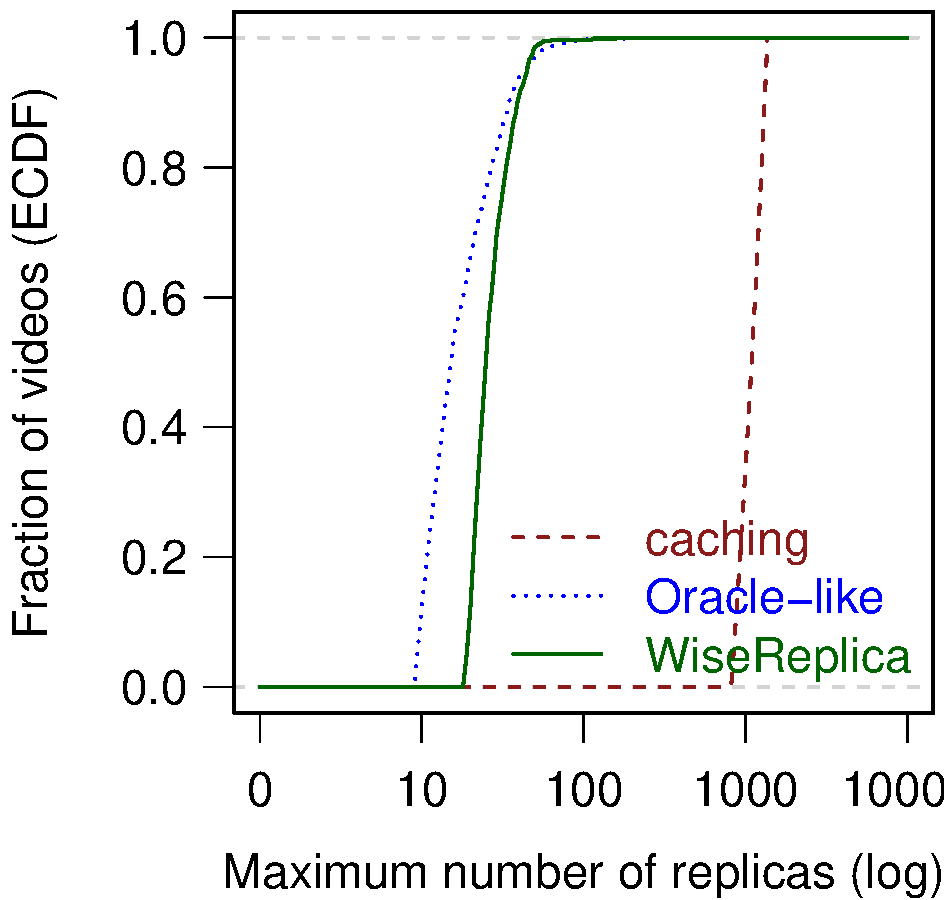
\includegraphics[width=.95\textwidth]{inputs/img/ecdf_replicas}
		\caption{The maximum number of replicas for the 1\% most popular videos.}
		\label{fig:replication_for_most_popular}
  %\centering
	\end{minipage}
	\hspace{0.1cm}
	\begin{minipage}[t]{0.48\linewidth}
     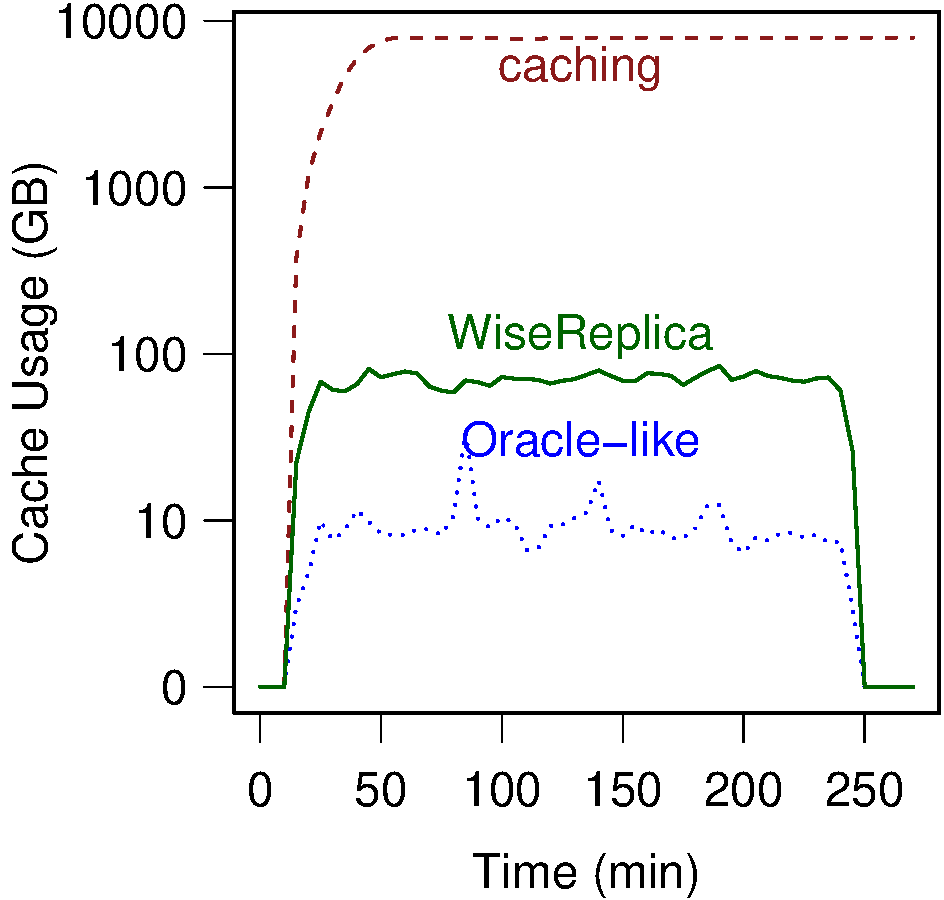
\includegraphics[width=.95\textwidth]{inputs/img/cache_usage}
		\caption{Storage usage for replication.}
		\label{fig:cache_usage_for_replication}
	\end{minipage}
\end{figure}

\subsubsection{Enhancing Bitrate Provision for Meeting Consumers' Expectation.}

\ WiseReplica performance is also quite similar to Oracle-like regarding preventing violations. Each point of the Figure~\ref{fig:violations} represents the number of SLA violations for intervals of five minutes. Overall, caching caused 7049 violations affecting 86\% of all viewers, WiseReplica had just 106 violations, and Oracle-like, evidently, none. Compared to caching, WiseReplica prevents nearly 99\% of violations. It copes with violations by (i) creating new replicas for hot videos only, and (ii) adapting the number of replicas according to the rank position. Vertical lines in Figure~\ref{fig:violations} represent the first access to the 10 videos with the worst content provision through caching. They account for 80.62\% of all caching violations. The appearance of these videos puts the system under heavy load, which makes caching fail to prevent violations.

Figure~\ref{fig:avg_bitrate} depicts the average bitrate for viewers of the 10 videos with the worst content provision using caching. When caching was under heavy load, half of viewers experienced a very low bitrate, ranging between 230Kbps and 2575Kbps. The mean bitrate with caching was 43Mbps. On average, WiseReplica improved this bitrate by roughly 85\% under heavy load. Actually it performs almost as well as the Oracle-like assumption, that improved bitrate provision by 93\%. These finds suggest that WiseReplica largely outperforms caching, fairly meeting consumers' expectations under heavy load conditions.

%\begin{figure}
%  \centering
%     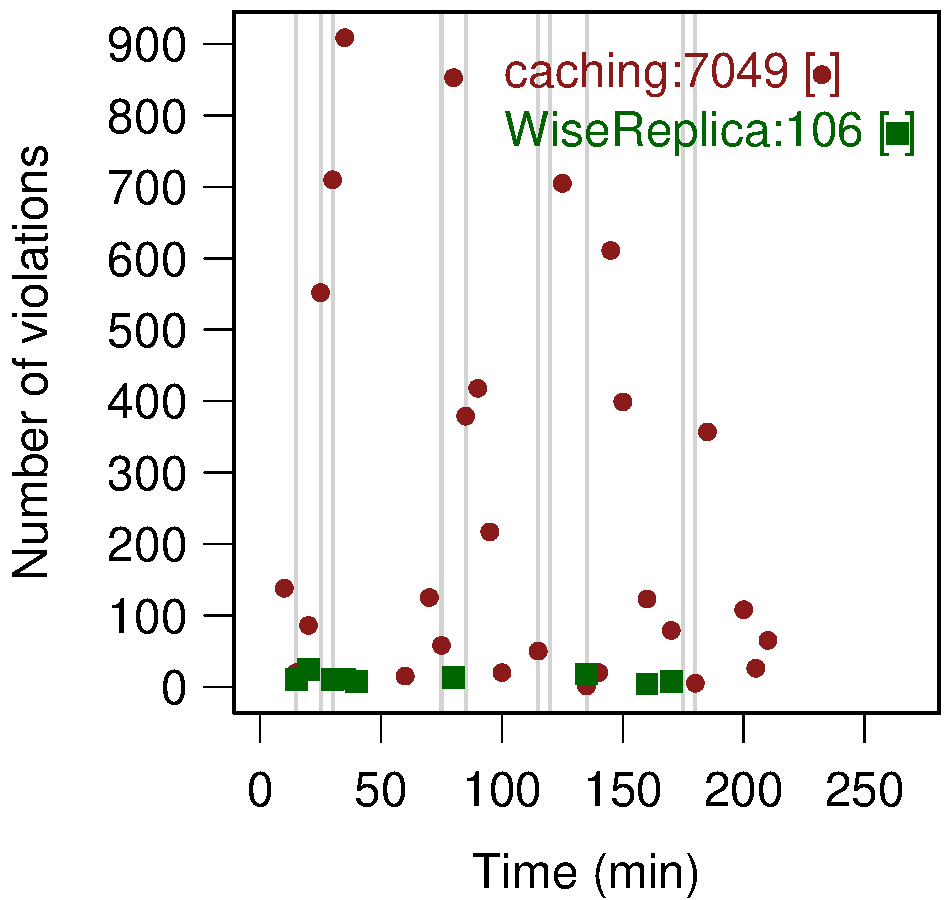
\includegraphics[width=.45\textwidth]{inputs/img/violations}
%  \caption{SLA violations. Vertical lines highlight the first view to 10 videos with the worst content provision using caching.}
%  \label{fig:violations}
%\end{figure}

\begin{figure}[htbp]
  \begin{minipage}[t]{0.48\linewidth}
     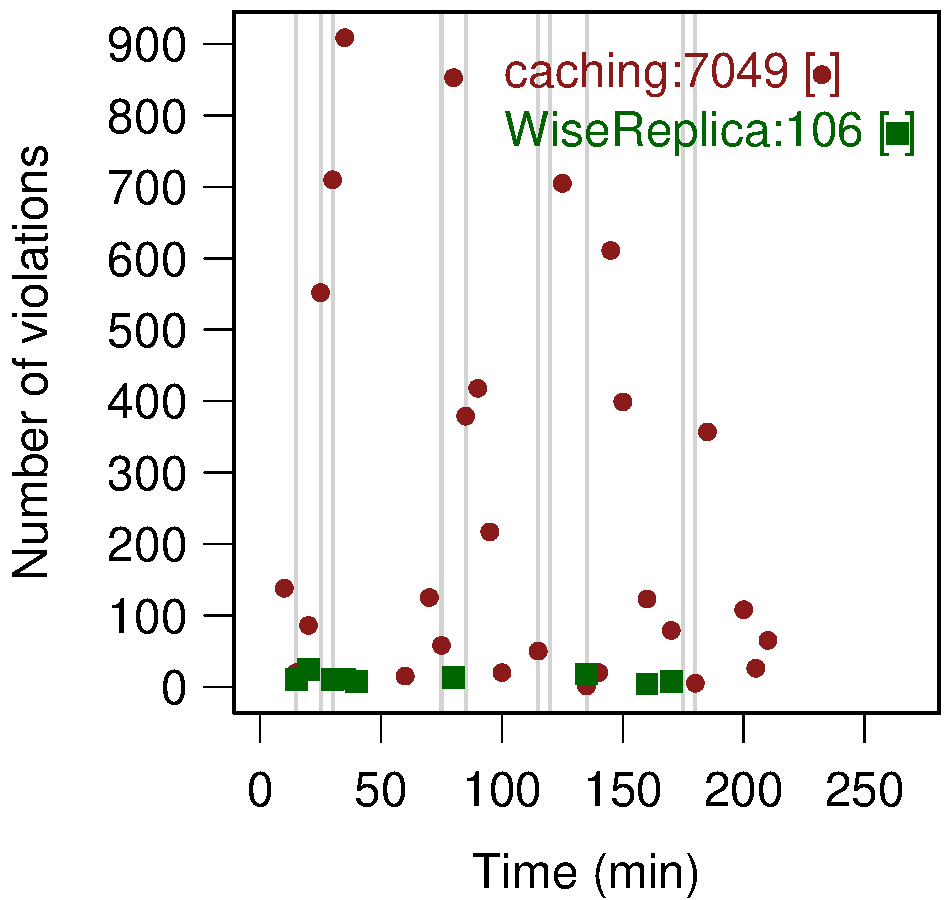
\includegraphics[width=.95\textwidth]{inputs/img/violations}
  \caption{SLA violations. Vertical lines highlight the first view to 10 videos with the worst content provision using caching.}
  \label{fig:violations}
  \end{minipage}
  \hspace{0.1cm}
  \begin{minipage}[t]{0.48\linewidth}
     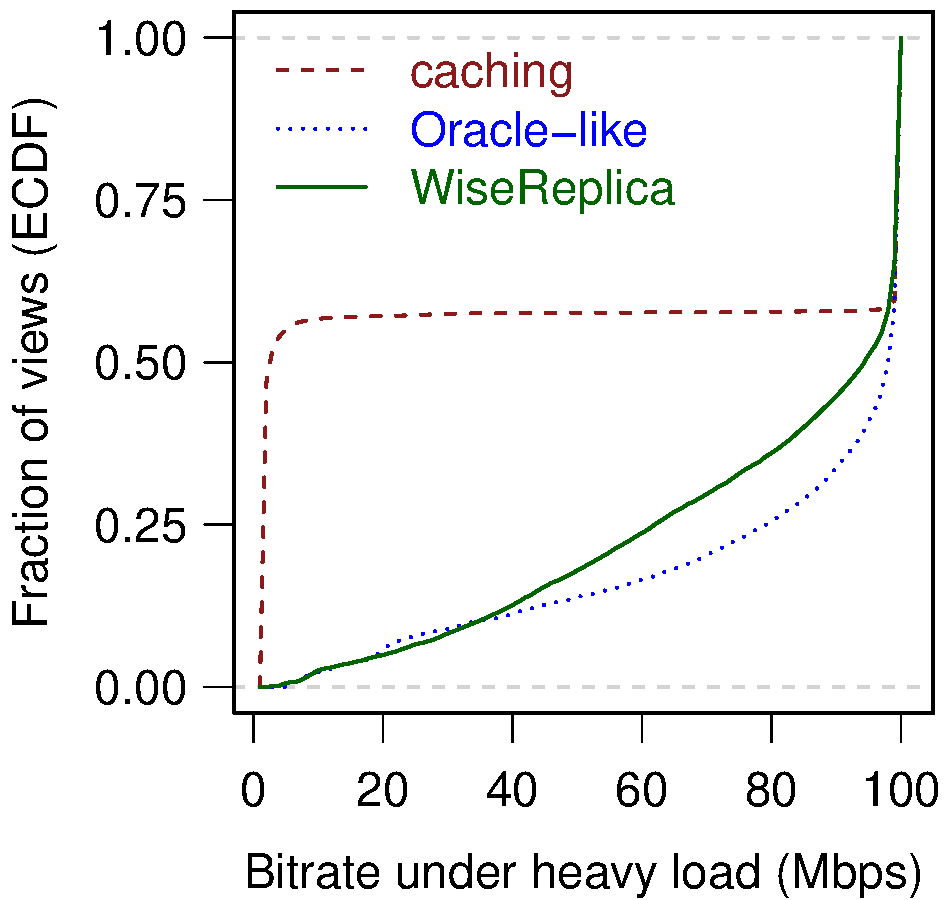
\includegraphics[width=.95\textwidth]{inputs/img/ecdf_agg_bwd_under_heavy_load}
  \caption{Bitrate for viewers of the 10 most popular videos under heavy load.}
  \label{fig:avg_bitrate}
  \end{minipage}
\end{figure}

\section{Related Work}
\label{sec:related_work}

Our related work is two-fold: Internet videos and adaptive replication schemes.

\noindent \textbf{Internet videos:} Recent studies
\cite{youtube_wsdm_2011,popularity_prediction_2010} have drawn
attention to reach a better understanding of Internet videos
properties, such as popularity growth. They point out that well-known
popularity characteristics are applicable to multimedia content. For
instance, Internet videos popularity distribution follows power law,
and popularity bursts have a short duration and are quite likely to
happen just after the content publication. Dobrian \emph{et
al.}~\cite{Dobrian_sigcomm_2011} shed some light on the performance of
Internet videos provision on CDNs. They show that average bitrate plays
an important role in videos availability. A hybrid solution between
CDNs and P2P is presented by Mansy \emph{et
al.}~\cite{Mansy_icnp_2011}. Their purpose is to model and analyze a
live video system and one of their main concerns is to adapt bitrate
for guarantee user satisfaction. Adhikari \emph{et
al.}~\cite{Adhikari_infocom_2012} work described the YouTube video
delivery system through measurements of DNS resolutions and video
playback traces. One of their findings is that over a globally
distributed network (PlanetLab) most part of the nodes have a nearby
Youtube video cache server to delivery the video data.  Moreover,
Brodersen \emph{et al.}~\cite{Brodersen_www_2012} presented a detailed
study over the strong connection between popularity and geographic
locality of Youtube videos. These facts endure our decision of a
locality aware solution for infrastructure. Liu \emph{et
al.}~\cite{Liu_sigcomm_2012} make a case for a video control plane
that can use a global view of client and network conditions to
dynamically optimize the video delivery in order to provide a high
quality viewing experience despite an unreliable delivery
infrastructure. However, the granularity of their server selection
mechanism is at a CDN, ignoring edge network resources. WiseReplica
addresses this issue by adapting replication close to the viewers.
Thus, WiseReplica can be play an important role in collaborating with an
Internet control plane.


\noindent
\textbf{Adaptive replication schemes:} Non-collaborative caching remains the simplest approach to provide popularity-aware replication of web content through cache replacement policies\cite{popularity_awaregreedydual_size_icdcs99}. However, we showed when we adapt the number of replicas according to the Internet video popularity properly, cache replacement policy becomes redundant. EAD \cite{Haiying_Shen_P2P_2010}
and Skute \cite{self_tolerant_acm_cloud_2010} adapt the number of replicas by
using a cost-benefit approach over decentralized and structured P2P
systems. EAD creates and deletes replicas throughout the query path
with regard to object hit rate using an exponential moving average
technique. Similarly, Skute provides a replication management scheme that
evaluates replicas price and revenue across different geographic
locations. Despite presenting an
efficient framework for replication, they provide an inaccurate bitrate provision, hence
inappropriate for high-quality video delivery. WiseReplica copes with this issue through analysing the request arrival process, performing accurate predictions about the ranking of Internet videos, and maintaining replication degree accordingly.

\section{Conclusions}
\label{sec:conclusion}

In this work, we presented WiseReplica, a SLA-based, adaptive replication scheme for meeting customers' expectations and enhancing resource allocation in peer-assisted VoD systems. To adapt replication, we proposed an accurate learning model for ranking Internet videos in order of \emph{hotness}. Our intuitive model is flexible, and can learn from different sources and big amounts of data, providing a robust framework for controlling VoD resource allocation. Simulations using YouTube traces suggest that predictions are important to enhance VoD delivery, allowing to self-adapt replication degree to video demand properly. WiseReplica increases the average bitrate provision by roughly 85\%, contributing decisively to enhance viewing experience of users. Our future work will mainly cover a proof-of-concept prototype for evaluating WiseReplica in a real testbed.



%most common style
%\bibliographystyle{plain}
%%%%%%%%%%%%%%%%%%%%%%%%%%%%%%%%%%%%%%%%%%%%%%
%well-organized, abbreviated bibliography style
%%%%%%%%%%%%%%%%%%%%%%%%%%%%%%%%%%%%%%%%%%%%%%
\bibliographystyle{abbrv}
\bibliography{inputs/biblio.bib}


\end{document}
